\documentclass[a4paper,10pt]{article}

\usepackage[margin=0.82in]{geometry}
\usepackage{amsmath,amssymb,amsthm,mathtools,bm}
\usepackage{graphicx}
\usepackage{booktabs}
\usepackage{array}
\usepackage{enumitem}
\usepackage{algorithm}
\usepackage{algpseudocode}
\usepackage{caption}
\usepackage{subcaption}
\usepackage{float}
\usepackage{microtype}
\usepackage{hyperref}
\usepackage{xcolor}
\usepackage{tikz}
\usetikzlibrary{arrows.meta,positioning}

\hypersetup{
  colorlinks=true,
  linkcolor=blue!55!black,
  citecolor=blue!55!black,
  urlcolor=blue!55!black
}

\setlength{\parindent}{0pt}
\setlength{\parskip}{0.35em}
\setlist[itemize]{leftmargin=1.5em,itemsep=0.15em,topsep=0.25em}
\setlist[enumerate]{leftmargin=1.7em,itemsep=0.15em,topsep=0.25em}

\newtheorem{remark}{Remark}
\newtheorem{assumption}{Assumption}
\newtheorem{proposition}{Proposition}

\newcommand{\E}{\mathbb{E}}
\newcommand{\Pbb}{\mathbb{P}}
\newcommand{\R}{\mathbb{R}}
\newcommand{\F}{\mathcal{F}}
\newcommand{\N}{\mathcal{N}}
\newcommand{\dd}{\mathrm{d}}
\newcommand{\diag}{\mathrm{diag}}
\newcommand{\bpi}{\bm{\pi}}
\newcommand{\bmu}{\bm{\mu}}
\newcommand{\bb}{\bm{b}}
\newcommand{\bg}{\bm{g}}
\newcommand{\bu}{\bm{u}}
\newcommand{\bw}{\bm{w}}
\newcommand{\bSigma}{\bm{\Sigma}}
\newcommand{\brho}{\bm{\rho}}
\newcommand{\bone}{\bm{1}}
\newcommand{\bB}{\bm{B}}
\newcommand{\bBh}{\widehat{\bm{B}}}
\newcommand{\bS}{\bm{S}}
\newcommand{\cH}{\mathcal{H}}
\newcommand{\imgorplaceholder}[3]{%
  \IfFileExists{#3}{\includegraphics[width=#1,height=#2,keepaspectratio]{#3}}{%
    \fbox{\parbox[c][#2][c]{#1}{\centering Missing figure\\[0.3em]\texttt{\detokenize{#3}}}}}%
}

\newcommand{\ICAPaperTitle}{Structure-Guided Reinforcement Learning for Partially Observed\\
Multi-Period Portfolio Optimization with Transaction Costs}
\newcommand{\ICAAuthorName}{Takahiro Kobayashi}
% Replace this with the official ICA session title once assigned, if it differs from the paper title.
\newcommand{\ICASessionTitle}{\ICAPaperTitle}
% Add the company or organizational affiliation before final submission if required.
\newcommand{\ICAAffiliation}{}

\title{\ICAPaperTitle}
\author{\ICAAuthorName}
\date{}

\begin{document}

\hypersetup{pageanchor=false}
\begin{titlepage}
\thispagestyle{empty}
\centering
\vspace*{1.5cm}
{\Large\bfseries \ICASessionTitle\par}
\vspace{1.2cm}
{\large Prepared by \ICAAuthorName\par}
\vfill
{\large Presented to the\par}
\vspace{0.35cm}
{\Large\bfseries 33rd International Congress of Actuaries (ICA2026)\par}
\vspace{0.35cm}
{\large November 8th--13th, 2026\par}
\vspace{0.45cm}
{\small\itshape July 29, 2026\par}
\vfill
\begin{minipage}{0.88\textwidth}
\small
This paper has been prepared for the 33rd International Congress of Actuaries.

The Institute of Actuaries of Japan (IAJ) and the International Actuarial Association (IAA) assume no responsibility for opinions or content expressed in this paper or in the accompanying materials. Furthermore, the opinions and content contained herein do not reflect the views of the IAJ or the IAA.

\vspace{0.8em}
\ICAAuthorName

\vspace{0.8em}
The IAJ and the IAA will ensure that all reproductions of the paper acknowledge the author(s) and include the above copyright statement.
\end{minipage}
\vfill
\end{titlepage}

\hypersetup{pageanchor=true}
\pagenumbering{arabic}
\maketitle

\begin{abstract}
This paper develops a structure-guided reinforcement-learning framework for multi-period portfolio optimization under latent market regimes and proportional transaction costs. The central theoretical contribution is a belief-state formulation of an entropy-regularized, precommitted mean--variance control problem: under common observation covariance, Wonham filtering reduces partial observation to a fully observed belief-state diffusion, and the associated Hamilton--Jacobi--Bellman (HJB) equation identifies a Gaussian exploratory policy and a wealth-quadratic value function; this structure is then extended to regime-dependent covariance by combining an exact Gaussian Bayes correction for a discretized observation model with a moment-matched control approximation. This theoretical reduction motivates a low-dimensional actor--critic (Stage~1) in place of an unrestricted state-to-weight learner, with regime-dependent parameter estimates supplied to the online filter by a statistical jump model. Building on the frozen Stage~1 policy as a state-dependent center, Stage~2 addresses transaction costs by learning asymmetric no-trade boundaries through direct pathwise optimization of a transaction-cost-aware terminal objective; this Direct Boundary policy optimization is motivated by, but is not a numerical solution of, a transaction-cost quasi-variational-inequality (QVI) benchmark, since joint critic--intervention learning of that QVI proved numerically unstable.

The common-covariance Stage~1 and Stage~2 policies are evaluated across five independent training seeds on a common set of $1000$ held-out paths. The Stage~1 policy is highly stable, with mean terminal wealth $1.1811$ and a 95\% Student-$t$ training-seed interval of $[1.1808,1.1814]$. The Direct Boundary policy achieves mean net terminal wealth $1.2009$ with interval $[1.1807,1.2211]$, exceeds daily center rebalancing by $0.0910$ with interval $[0.0709,0.1112]$, and reduces the mean trade count from $252$ to $175.8$ under the evaluated band-plus-leverage-cap policy. Its descriptive difference from Stage~1 net terminal wealth is $0.0198$ with interval $[-0.0003,0.0400]$; because this interval includes zero and the two stages optimize different objectives, no Stage~1-versus-Stage~2 dominance claim is made. The regime-dependent-covariance extension remains a single-seed exploratory result outside this five-seed robustness analysis. The framework is presented as a portfolio-control building block for institutional and actuarial applications rather than a complete asset--liability management model.
\end{abstract}

\noindent\textbf{Keywords:} continuous-time reinforcement learning; mean--variance portfolio selection; partial information; regime switching; transaction costs; no-trade region; actor--critic.

\section{Introduction}

Dynamic portfolio choice becomes substantially harder when three realistic features are introduced simultaneously: investment opportunities vary across persistent market regimes, the regime is not directly observed, and trading incurs transaction costs. Partial information requires the investor to infer the state of the market from prices. Multi-period objectives require decisions to account for their effect on future wealth and information. Transaction costs make frequent rebalancing suboptimal and typically replace frictionless point targets by state-dependent no-trade regions. These features lead naturally to stochastic filtering, nonlinear dynamic programming, and high-dimensional policy optimization.

The starting point of this study is the natural compatibility between portfolio choice and reinforcement learning. A portfolio rule is a policy that maps an information state into an asset allocation, while reinforcement learning is designed to learn state-dependent sequential decisions from interaction data. The central issue is therefore not only which learning algorithm to use, but also how to construct the state, policy class, and objective. Here financial domain knowledge enters all three components: filtering converts return histories into an economically interpretable regime belief; stochastic-control theory restricts the actor and critic to HJB-consistent forms; and the objective incorporates target wealth, exploration, turnover, and transaction costs. This structure is intended to improve sample efficiency, numerical stability, and interpretability relative to an unrestricted state-to-weight learner. The five-seed common-covariance experiments assess robustness to training initialization, but they do not isolate the contribution of each structural restriction through a controlled structured-versus-unstructured ablation; repeated-seed robustness and ablation are distinct open questions.

This compatibility does not imply that reinforcement learning is necessary for every low-dimensional portfolio problem. Its role here is computational: it provides a simulation-based policy-approximation method when partial information, nonlinear objectives, and transaction costs make direct dynamic programming difficult to implement.

This restriction is particularly important in regime-switching markets. Abrupt changes, persistent latent states, noisy regime estimates, and delayed terminal rewards can make generic deep-RL policies difficult to train. Preliminary experiments with less structured deep architectures, including Transformer-style state encoders and an unrestricted transaction-cost policy, did not yield a sufficiently reliable policy for the reported study. These trials do not isolate a single cause: policy-class flexibility, terminal credit assignment, state normalization, pathwise-gradient variance, hyperparameters, and training budget may all contribute. Constraining the output to economically meaningful, center-relative policy geometry provided a stronger inductive bias. The project therefore uses financial mathematics to determine the belief state and feasible policy geometry, while leaving only lower-dimensional coefficients or boundaries to be learned. For the costly problem, the frictionless solution is used as an advanced start so that Stage~2 learns a correction around an economically meaningful benchmark rather than the full policy from scratch.

Regime changes are also not limited to expected returns. Volatility levels and cross-asset correlations can change materially across market conditions, and these covariance shifts directly affect diversification, risk budgets, capital requirements, and the scale of admissible positions. For practical portfolio and risk management, covariance misspecification may therefore be at least as consequential as drift misspecification. This motivates the regime-dependent-covariance extension, while the common-covariance model is retained as the theorem-level benchmark needed to identify which HJB structures can be transferred safely.

This paper combines two complementary components. Stage~1 learns a frictionless portfolio policy under partial information. It starts from the continuous-time precommitted mean--variance formulation of Wu and Li~\cite{wu2024}, extends its structured actor--critic representation to multiple risky assets, and makes the filtering, policy, value function, and learning pipeline operational. Stage~2 first formulates the transaction-cost problem as a QVI on the enlarged state $(t,x,p,w)$. Because the corresponding critic-based implementation was not numerically stable in the current experiments, the reported method uses Center+DNNBand, a policy trained by \emph{Direct Boundary policy optimization}: a critic-free method in which a neural policy predicts lower and upper no-trade boundaries around the frozen Stage~1 center and is trained by pathwise differentiation directly through the wealth recursion with proportional costs, rather than through a learned value function. We refer to this evaluated policy as Center+DNNBand throughout the remainder of the paper. The reported Stage~2 does not claim to solve the exact transaction-cost extension of the Stage~1 mean--variance problem: it uses the Stage~1 policy as a state-dependent structural feature and optimizes a separate transaction-cost-aware terminal objective.

The organizing principle is \emph{structure-guided learning}. In Stage~1, the observable state is determined by filtering, the exploratory policy family is determined by the HJB, and the critic is restricted by the quadratic terminal condition. In Stage~2, classical transaction-cost theory motivates an inaction region, while the Stage~1 policy supplies a state-dependent anchor. Learning is therefore used to estimate a small set of economically meaningful objects rather than an unrestricted state-to-action map.

Across the contributions, the common methodological principle is selective function approximation: low-dimensional parametrization is used where the control equation identifies the policy form, while neural approximation is reserved for residual boundary geometry that remains analytically unresolved. The distinction between the two stages is therefore not simply parametric learning versus deep learning; it reflects how sharply the underlying control theory identifies the admissible functional form.

The paper makes the following contributions.
\begin{enumerate}[label=(\roman*)]
\item \textbf{A belief-state Hamilton--Jacobi--Bellman (HJB) reduction of partially observed mean--variance control, including a regime-dependent-covariance extension.} Under common observation covariance, Wonham filtering reduces the partially observed control problem to a fully observed diffusion on the belief state, and the entropy-regularized HJB equation for this belief-state problem admits a closed-form Gaussian exploratory policy together with a wealth-quadratic value function solving a lower-dimensional coefficient PDE system. We extend this reduction to regime-dependent covariance by combining an exact Gaussian Bayes correction for a discretized hidden-Markov observation model with a moment-matched, belief-averaged control approximation, deriving the resulting approximate HJB, Gaussian policy, and coefficient equations, including the additional nonlinear term that vanishes in the common-covariance benchmark. This is the central theoretical contribution of the paper; no verification or approximation-error theorem is claimed for the regime-dependent extension, and its supporting numerical experiment is a separate single-seed exploratory result outside the paper's five-seed robustness analysis.

\item \textbf{A structure-guided actor--critic implementation of the belief-state HJB reduction (Stage~1).} We make the multi-asset belief-state actor--critic operational: the Gaussian policy family, its wealth-linear mean, and the wealth-quadratic critic are fixed by the HJB reduction above, so learning is restricted to a low-dimensional set of belief/time coefficients rather than an unrestricted state-to-weight map. Regime-specific drift, covariance, and transition-intensity estimates are supplied to the online Bayesian filter by a statistical jump model applied to persistent offline labels, integrating an established regime-identification method with the HJB-guided control pipeline rather than proposing new SJM statistical theory.

\item \textbf{A two-stage transaction-cost architecture with a learned no-trade boundary (Stage~2).} We formulate the costly extension of the Stage~1 problem as a quasi-variational inequality (QVI) on the enlarged state $(t,x,p,\bw)$ and derive a center-relative critic/intervention parametrization consistent with its continuation and intervention structure. Because joint QVI-residual and intervention learning was numerically unstable, the reported implementation retains the QVI's robust structural implications---a frictionless center, an inaction region, feasibility constraints, and pathwise transaction costs---and learns asymmetric no-trade boundaries directly around the frozen Stage~1 center through Direct Boundary policy optimization: a critic-free method that optimizes a separate transaction-cost-aware terminal objective by differentiating directly through simulated wealth paths. The QVI remains the theoretical benchmark and a target for future stabilization work, not a claim that the reported boundary policy solves it.

\item \textbf{A TD-inspired implementation refinement for continuous-time actor--critic learning.}
The Stage~1 actor update combines a local martingale increment, which plays a temporal-difference-like role, with a normalized full-horizon tail residual, which provides a Monte Carlo-like terminal correction. Together with the critic update, this mixed signal is designed to address finite-horizon credit assignment and provided a usable implementation in the reported experiments. It is presented as an algorithmic refinement rather than a new continuous-time RL theorem; a controlled actor-signal ablation remains to be completed.
\end{enumerate}

The Stage~1 and Stage~2 architectures above are empirically validated across five independent training seeds, each evaluated on a common set of $1000$ independently generated held-out paths. For each training seed, the same fixed evaluation scenarios are used to compute seed-level summary statistics; these are then combined across seeds into a mean, a between-seed standard deviation, and a 95\% Student-$t$ interval with four degrees of freedom. Where two policies are compared on the same paths, paired differences are computed at the evaluation-episode level before aggregation across seeds. This design quantifies sensitivity to training initialization under a fixed market-evaluation design; it is not a claim about market-distribution uncertainty. Under this protocol, the Stage~1 policy is extremely stable across training seeds, while Stage~2 shows materially greater training-seed variability. The regime-dependent-covariance extension in contribution (i) is not part of this five-seed validation and is reported separately as a single-seed exploratory result.

\subsection*{Actuarial relevance and potential applications}
\label{sec:actuarial}

The framework is motivated by long-horizon institutional investment problems faced by insurers, pension funds, and other liability-aware investors. In such settings, the economically relevant decision is not only the current asset allocation but also the future sequence of rebalancing decisions. Market conditions are persistent but not directly observable, parameter estimates are noisy, and large investors face bid--ask spreads, commissions, market impact, operational constraints, and governance limits on trading frequency. These features make partial information and transaction costs central rather than secondary modeling details.

The target terminal wealth $z$ can be interpreted as a reduced-form funding or accumulation target related to future benefit payments, a required funding ratio, a credited-rate objective, or a long-term reserve target. The belief $p_t$ provides an explicit summary of uncertainty about the prevailing market environment, while a no-trade region translates the trade-off between tracking a desired allocation and avoiding unnecessary turnover into an explainable decision rule. This is potentially useful in settings where investment policies must be communicated to risk committees and implemented subject to transaction and governance budgets.

The present model is not a full asset--liability management model. It does not include stochastic liabilities, solvency capital, regulatory constraints, cash-flow matching, or liability-dependent utility. Instead, it provides a portfolio-control building block that could be embedded in a broader ALM framework by replacing the terminal target and admissible set with liability- and capital-sensitive specifications.

Table~\ref{tab:positioning} summarizes how the main components are positioned relative to prior literature. The table supplements, rather than replaces, the contribution statements above.

\begin{table}[H]
\centering
\small
\caption{Positioning of the paper relative to prior literature.}
\label{tab:positioning}
\begin{tabular}{>{\raggedright\arraybackslash}p{0.20\textwidth} >{\raggedright\arraybackslash}p{0.34\textwidth} >{\raggedright\arraybackslash}p{0.38\textwidth}}
\toprule
Component & Prior literature & This paper \\
\midrule
Stage~1 control & One-risky-asset hidden-regime benchmark; common-covariance multi-asset extension & Operational multi-asset actor--critic with explicit coefficient PDEs and implementation details \\
Regime estimation & SJM-based persistent regime identification & SJM labels integrated into parameter estimation for online belief-state control \\
Covariance structure & Common observation covariance in the theorem-level benchmark & Discretized Markov prediction and exact Gaussian Bayes correction plus an approximate belief-averaged HJB control layer \\
Transaction costs & Classical no-trade regions and HJB-initialized boundary networks & Belief-conditioned two-stage learning with a frozen Stage~1 center and Center+DNNBand \\
Actor update & Martingale-based continuous-time policy evaluation and gradient methods & Mixed local martingale and full-horizon rollout signal for finite-sample learning \\
\bottomrule
\end{tabular}
\end{table}

\section{Related Literature}

\subsection{Continuous-time reinforcement learning and mean--variance control}

The continuous-time reinforcement-learning foundation used here follows the exploratory stochastic-control formulation of Wang, Zariphopoulou, and Zhou~\cite{wangzariphopoulouzhou2020}. Randomized controls and entropy regularization convert exploration into part of the control objective. In linear--quadratic problems, this construction naturally produces Gaussian policies. Wang and Zhou~\cite{wangzhou2020} apply the framework to continuous-time mean--variance portfolio selection and show how analytical structure can substantially reduce the number of learned parameters.

Jia and Zhou~\cite{jiazhope2022} develop a martingale characterization of continuous-time policy evaluation. A central insight is that a naive mean-square temporal-difference error converges toward quadratic variation and is not, by itself, the appropriate continuous-time value-fitting objective. They instead derive martingale-loss and martingale-orthogonality formulations that recover continuous-time analogues of Monte Carlo and TD methods. Their companion paper~\cite{jiazhopepg2022} derives policy-gradient representations and offline and online actor--critic algorithms. The policy-gradient problem is recast through policy evaluation, while online updates use martingale orthogonality and stochastic approximation. These results motivate the martingale-based critic and actor signals used in Stage~1.

\subsection{Partial information and regime-switching portfolios}

Partial-information portfolio problems separate state estimation from control when an appropriate filtering reduction is available. Wonham~\cite{wonham1964} derives the finite-state nonlinear filter used in the common-covariance benchmark, while Krishnamurthy~\cite{krishnamurthy2016} develops the broader POMDP perspective in which the posterior distribution becomes the fully observed belief state. Xiong and Zhou~\cite{xiongzhou2007} establish a separation principle for continuous-time mean--variance selection under partial information, and Elliott, Siu, and Badescu~\cite{elliott2010} study estimation and filtering under hidden Markov regimes.

For observable market regimes, Zhou and Yin~\cite{zhouyin2003} derive continuous-time mean--variance results and efficient-frontier implications. Under unobservable Markov-modulated drift, Rieder and B{\"a}uerle~\cite{rieder2005} study portfolio optimization after filtering and identify the interaction between current opportunities and hedging against belief changes. These papers clarify the role of regime information and motivate the myopic--hedging decomposition used in the present Stage~1 actor.

The closest benchmark is Wu and Li~\cite{wu2024}. They formulate an entropy-regularized, precommitted mean--variance problem with an unobservable market regime, use Wonham filtering to obtain a belief-state problem, and derive semi-analytical representations of the value function and Gaussian optimal policy. The unknown coefficient functions solve lower-dimensional parabolic PDEs and are approximated by polynomials inside an actor--critic algorithm. The present Stage~1 follows this logic, makes the multi-asset extension explicit, and adds a practical regime-estimation pipeline and a regime-dependent covariance experiment.

\subsection{Statistical jump models for regime identification}

Statistical jump models estimate persistent market regimes by clustering temporally constructed features while directly penalizing changes in the latent label sequence. This formulation offers a non-likelihood-based alternative to a conventional hidden Markov model and is particularly attractive when financial regimes are persistent, imbalanced, or supported by limited data. Ayd{\i}nhan, Kolm, Mulvey, and Shu~\cite{aydinhan2024} review the discrete statistical jump model and extend its discrete hidden state to a probability vector on the regime simplex. Their continuous statistical jump model introduces smooth regime probabilities, derives a probabilistic interpretation of the transition penalty, and adds a mode-loss penalty that encourages decisive regime assignments. Their simulations and market experiments report improved robustness relative to discrete jump models and standard HMM estimation, especially under regime imbalance and short samples.

The present paper uses the simpler discrete two-state SJM rather than the continuous extension of Ayd{\i}nhan et al. Its role is also narrower: the SJM provides a persistent offline segmentation from which regime-specific drifts, covariances, and empirical transition rates are estimated. It does not replace the online Wonham or Gaussian Bayes filter used to construct the belief state for control. Thus, the contribution here is the integration of SJM-based estimation with an HJB-guided portfolio-learning architecture, not a new SJM estimator or a new statistical consistency result.

The choice of SJM does not imply that it uniformly dominates hidden Markov models. HMMs provide a coherent probabilistic observation model and naturally generate filtered and smoothed regime probabilities. The discrete SJM used here instead offers direct control over label persistence through the jump penalty and produces regime prototypes in an economically constructed feature space. This makes the persistence penalty, feature centroids, and resulting offline segmentation particularly transparent when the objective is to identify persistent regimes rather than to estimate a complete generative return model.

The two approaches play complementary roles in the present pipeline. SJM is used offline to segment historical or simulated observations and estimate regime-dependent moments and transition intensities. Online allocation does not treat the resulting hard SJM label as an observed state; it uses a Bayesian filter to update the posterior regime probability from newly observed returns. This separation avoids supplying an ex-post label directly to the controller and preserves the partial-information structure of the investment problem.

\subsection{Transaction costs and no-trade regions}

The no-trade-region principle originates in classical proportional-cost portfolio theory. Magill and Constantinides~\cite{magill1976} show that investors optimally tolerate deviations from frictionless target proportions. Davis and Norman~\cite{davisnorman1990} provide a rigorous infinite-horizon formulation and numerical characterization, and Shreve and Soner~\cite{shrevesoner1994} establish existence, uniqueness, and regularity results using viscosity-solution methods. Taksar, Klass, and Assaf~\cite{taksar1988} provide a diffusion model with brokerage fees in which the risky-to-safe wealth ratio is kept inside an interval with the minimum intervention needed at its boundaries. Together, these studies supply the economic and QVI intuition for Stage~2: proportional costs create an inaction region rather than a continuously tracked point target.

High-dimensional PDE methods motivate neural approximations when grid-based QVI solvers become impractical. Han, Jentzen, and E~\cite{han2018} and Sirignano and Spiliopoulos~\cite{sirignano2018} develop deep-learning methods for high-dimensional PDEs. In portfolio optimization, Mulvey et al.~\cite{mulvey2020} solve a frictionless HJB system for mean-reverting Ornstein--Uhlenbeck assets to obtain an advanced start and then use a feedforward neural network to approximate state- and time-dependent no-trade boundaries. Their experiments demonstrate scalability to high-dimensional collections of correlated pair trades. The present work adopts the same broad principle---combine a tractable frictionless solution with a learned transaction-cost correction---but differs in three respects. The underlying market is regime-switching rather than OU, the state contains a filtered belief, and the reported Stage~2 network directly optimizes a separate terminal utility and regularization objective through simulated wealth paths. Accordingly, the Stage~1 center is a structural feature rather than the exact zero-cost optimizer of the Stage~2 objective.

\section{Decision Framework and Partially Observed Market}

\subsection{From partial observation to belief-state control}

A reinforcement-learning problem is described by an information state, an action, a policy, and an objective. In this portfolio application, the action is an allocation of risky exposure, while the information state must summarize what is relevant for both future wealth dynamics and future decisions. In Stage~1 the observable control state is $(t,X_t,p_t)$, where $X_t$ is discounted wealth and $p_t$ is the posterior probability of regime~1. In Stage~2 the current holdings or portfolio weights are added because transaction costs depend on the distance between pre-trade and post-trade positions.

The underlying regime $I_t$ is not observed directly. The investor observes the price or return history $\F_t^S$, so the original problem is a partially observed Markov decision process. Under the filtering assumptions used below, the posterior distribution of the finite-state regime is a sufficient statistic for that observation history. The problem can therefore be reformulated as a fully observed Markov control problem on the \emph{belief state}~\cite{krishnamurthy2016}. This transformation does not eliminate regime uncertainty: it represents that uncertainty explicitly through
\begin{equation}
p_t=\Pbb(I_t=1\mid\F_t^S).
\end{equation}
The belief is thus an information state for control, not merely a regime-classification score.

The actor specifies the portfolio decision conditional on the information state. The critic approximates the conditional expected continuation objective from that state, and actor--critic learning uses the critic signal to improve the actor. Reinforcement learning is employed here as a simulation-based numerical approximation method; stochastic filtering and control theory determine the state representation and restrict the functional forms being learned.

\begin{table}[H]
\centering
\small
\caption{Reinforcement-learning objects in the portfolio-control problem.}
\label{tab:rl_correspondence}
\begin{tabular}{>{\raggedright\arraybackslash}p{0.17\textwidth} >{\raggedright\arraybackslash}p{0.35\textwidth} >{\raggedright\arraybackslash}p{0.37\textwidth}}
\toprule
Object & Stage~1: frictionless control & Stage~2: costly rebalancing \\
\midrule
Information state & $(t,X_t,p_t)$ & $(t,X_t,p_t,\bw_t)$ \\
Action & Risky-dollar position $\bu_t$ & Post-trade weight or intervention target \\
Actor / policy & Gaussian distribution conditional on the belief state & Belief- and horizon-dependent no-trade boundaries \\
Critic / value model & Expected exploratory mean--variance cost-to-go & QVI value function in the theoretical design; no separate critic in the reported Direct Boundary implementation \\
Learning objective & Martingale and terminal cost-to-go signals & Differentiable terminal utility plus turnover, gap, and leverage regularization \\
Learning role & Estimate low-dimensional policy and value coefficients & Estimate boundary geometry around the frozen Stage~1 center \\
\bottomrule
\end{tabular}
\end{table}

Figure~\ref{fig:belief_control_flow} summarizes the information flow. The hidden regime affects observed returns but is not supplied directly to the controller. The filter compresses the observation history into $p_t$, which enters the state used by the actor or boundary policy.

\begin{figure}[H]
\centering
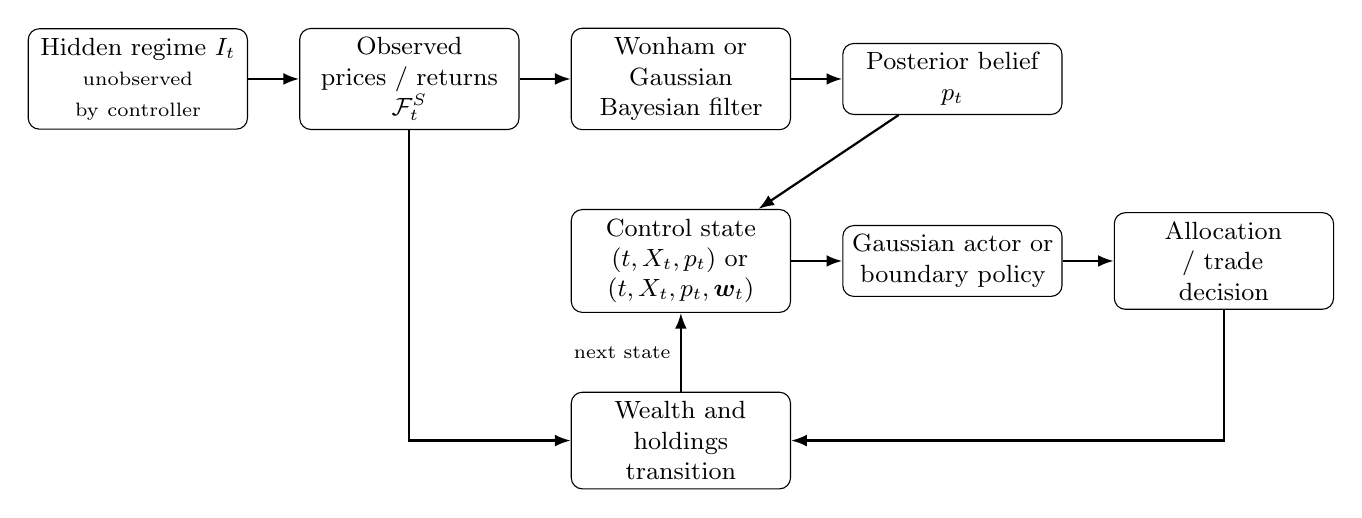
\begin{tikzpicture}[
  node distance=0.65cm and 0.65cm,
  box/.style={draw,rounded corners,align=center,minimum height=0.9cm,text width=2.55cm,font=\small},
  arrow/.style={-{Latex[length=2mm]},thick}
]
\node[box] (regime) {Hidden regime $I_t$\\{\scriptsize unobserved by controller}};
\node[box,right=of regime] (returns) {Observed prices / returns\\$\F_t^S$};
\node[box,right=of returns] (filter) {Wonham or Gaussian\\Bayesian filter};
\node[box,right=of filter] (belief) {Posterior belief\\$p_t$};
\node[box,below=1.0cm of filter] (state) {Control state\\$(t,X_t,p_t)$ or $(t,X_t,p_t,\bw_t)$};
\node[box,right=of state] (policy) {Gaussian actor or\\boundary policy};
\node[box,right=of policy] (action) {Allocation / trade\\decision};
\node[box,below=1.0cm of state] (transition) {Wealth and holdings\\transition};
\draw[arrow] (regime) -- (returns);
\draw[arrow] (returns) -- (filter);
\draw[arrow] (filter) -- (belief);
\draw[arrow] (belief) -- (state);
\draw[arrow] (state) -- (policy);
\draw[arrow] (policy) -- (action);
\draw[arrow] (action) |- (transition);
\draw[arrow] (returns) |- (transition);
\draw[arrow] (transition) -- node[left,font=\scriptsize] {next state} (state);
\end{tikzpicture}
\caption{Belief-state construction and portfolio-control information flow.}
\label{fig:belief_control_flow}
\end{figure}

\subsection{Selective use of deep function approximation}

Neural networks provide flexible approximations to high-dimensional nonlinear functions, but flexibility is not costless: a larger function class can increase optimization variance, data requirements, computational burden, and the difficulty of understanding the resulting decision rule. The present framework therefore does not use deep learning uniformly across the two stages. Model complexity is allocated according to the extent to which stochastic-control theory identifies the relevant functional form. Deep learning is not treated as inherently uninterpretable; interpretability depends substantially on what the network is permitted to represent.

In Stage~1, the HJB implies a Gaussian exploratory policy, a policy mean that is linear in wealth relative to the multiplier, and a value function that is quadratic in wealth. A low-dimensional parametrization is therefore used instead of a generic deep state-to-weight network. This choice preserves the analytically identified structure and avoids asking simulation data to relearn a functional form already supplied by the control problem. The principal motivations are identifiability, sample efficiency, and numerical discipline; reduced computation and improved interpretability are additional benefits rather than the primary justification.

In Stage~2, the transaction-cost QVI identifies the enlarged state, continuation-versus-intervention logic, proportional-cost wealth transition, and qualitative role of an inaction region around a frictionless center. It does not characterize the finite-horizon multidimensional lower and upper boundaries sufficiently sharply for the present implementation. The reported neural network is therefore not asked to learn an unrestricted portfolio policy. It learns only the residual time-, belief-, wealth-, and holdings-dependence of the boundaries, subject to center-relative geometry, ordering, and feasibility constraints. The architecture is thus structurally parametric in its economic geometry but flexible in the remaining state dependence.

\subsection{Regime-switching market}

The latent chain is a parsimonious representation of persistent market conditions, such as favorable versus stressed, risk-on versus risk-off, or normal versus high-volatility environments. It is not a literal claim that financial markets have only two economic states. A continuous-time Markov chain captures random switching while preserving tractability: $\lambda_i$ is the transition intensity out of regime $i$, and the expected holding time in that regime is $1/\lambda_i$. The two-state specification is adopted for interpretation and computational economy; additional states, duration dependence, or non-Markov persistence are possible extensions.

The economic labels are determined by the estimated drift and covariance parameters rather than imposed in advance. In the common-covariance benchmark only expected returns change by regime. The later extension also allows volatility and cross-asset correlation to change, reflecting their direct role in diversification and risk concentration.

Let $I_t\in\{1,2\}$ be a latent continuous-time Markov chain with generator
\begin{equation}
Q=
\begin{pmatrix}
-\lambda_1 & \lambda_1\\
\lambda_2 & -\lambda_2
\end{pmatrix},
\qquad \lambda_1,\lambda_2>0.
\label{eq:generator}
\end{equation}
There are $d$ risky assets and one risk-free asset with rate $r$. In the common-covariance benchmark,
\begin{equation}
\dd\bS_t
=\mathrm{Diag}(\bS_t)\bigl(\bmu_t\,\dd t+\sigma\,\dd\bB_t\bigr),
\qquad
\bmu_t=\bmu^{(1)}\bm{1}_{\{I_t=1\}}+\bmu^{(2)}\bm{1}_{\{I_t=2\}},
\label{eq:asset}
\end{equation}
where $\sigma\in\R^{d\times d}$ is nonsingular and $\bSigma=\sigma\sigma^\top$. Define
\begin{equation}
\brho^{(i)}=\sigma^{-1}(\bmu^{(i)}-r\bone),
\qquad i=1,2.
\end{equation}
If $\bu_t\in\R^d$ denotes discounted risky-dollar positions, discounted wealth under full information satisfies
\begin{equation}
\dd X_t^{u}=\bu_t^\top\sigma\bigl(\brho_t\,\dd t+\dd\bB_t\bigr).
\end{equation}

The regime is hidden. The investor observes prices and uses the posterior belief
\begin{equation}
p_t=\Pbb(I_t=1\mid\F_t^S).
\end{equation}
The original control problem is therefore a partially observed Markov decision problem. Under the common-covariance assumption, the posterior $p_t$ is a sufficient statistic for the observation history, so the POMDP is converted into a fully observed control problem on the belief state.

\begin{proposition}[Belief-state reduction under common covariance]
\label{prop:belief_reduction}
Suppose the regime follows \eqref{eq:generator}, the asset model is \eqref{eq:asset}, $\sigma$ is nonsingular and common across regimes, and controls are adapted to the price filtration. Then the innovation process in \eqref{eq:innovation} is Brownian with respect to that filtration, the posterior belief satisfies \eqref{eq:belief}, and discounted wealth satisfies \eqref{eq:wealth_observed}. Consequently, $(t,X_t,p_t)$ is a fully observed Markov information state for Stage~1.
\end{proposition}

\begin{proof}[Proof sketch]
Define the filtered drift and the innovation process by
\begin{equation}
\widehat{\bmu}(p)=p\bmu^{(1)}+(1-p)\bmu^{(2)},
\end{equation}
\begin{equation}
\dd\bBh_t
=\sigma^{-1}\dd\log\bS_t
-\sigma^{-1}\left(\widehat{\bmu}(p_t)-\tfrac12\diag(\bSigma)\right)\dd t.
\label{eq:innovation}
\end{equation}
Because the observation covariance is the same in both regimes, the innovations theorem implies that $\bBh$ is Brownian in the price filtration~\cite{wonham1964}. Indeed,
\begin{equation}
\dd\log\bS_t
=\left(\bmu_t-\tfrac12\diag(\bSigma)\right)\dd t+\sigma\dd\bB_t
=\left(\widehat{\bmu}(p_t)-\tfrac12\diag(\bSigma)\right)\dd t+\sigma\dd\bBh_t.
\end{equation}
Substituting this representation into discounted wealth and applying the two-state Wonham filter gives
\begin{align}
\dd X_t^{u}
&=\bu_t^\top\sigma\bigl(\widehat{\brho}(p_t)\,\dd t+\dd\bBh_t\bigr),
\label{eq:wealth_observed}\\
\dd p_t
&=a(p_t)\,\dd t+b(p_t)^\top\dd\bBh_t,
\label{eq:belief}
\end{align}
where
\begin{equation}
\widehat{\brho}(p)=p\brho^{(1)}+(1-p)\brho^{(2)},\quad
a(p)=\lambda_2-(\lambda_1+\lambda_2)p,\quad
b(p)=p(1-p)(\brho^{(1)}-\brho^{(2)}).
\end{equation}
Thus $(X_t,p_t)$ is the observable state for Stage~1. The shared innovation in \eqref{eq:wealth_observed}--\eqref{eq:belief} creates a wealth--belief cross-variation term in the HJB.
\end{proof}

For simulation with step $\Delta t$, the filter is implemented by a prediction--correction recursion. The Markov prediction is
\begin{equation}
p_{k\mid k-1}=p_{k-1}(1-\lambda_1\Delta t)+(1-p_{k-1})\lambda_2\Delta t.
\label{eq:common_prediction}
\end{equation}
Under the common-covariance observation model, the log-return likelihood is
\begin{equation}
y_k\mid I_k=i\sim\N\left(
\left(\bmu^{(i)}-\tfrac12\diag(\bSigma)\right)\Delta t,
\bSigma\Delta t
\right),
\end{equation}
and the two predicted log weights are normalized with a log-sum-exp calculation. The controller never observes $I_k$; it receives $(t_k,X_k,p_k)$.

\subsection{Exploratory mean--variance objective}

For a target expected terminal wealth $z$, the precommitted mean--variance problem is
\begin{equation}
\min_{\bu}\operatorname{Var}(X_T^u)
\quad\text{subject to}\quad \E[X_T^u]=z.
\end{equation}
Here ``precommitted'' means that the policy is selected at the initial date for the terminal mean--variance criterion and is not subsequently reoptimized as a time-consistent equilibrium strategy.
Introducing a Lagrange multiplier $\omega$ gives the saddle formulation
\begin{equation}
\sup_{\omega\in\R}\inf_{\bu}\left\{
\E[(X_T^u-\omega)^2]-(\omega-z)^2
\right\}.
\label{eq:mv_lagrange}
\end{equation}
For a fixed multiplier $\omega$, the inner control problem is the entropy-regularized problem developed below. The multiplier is subsequently updated by dual ascent so that the terminal-wealth mean constraint is satisfied; this outer step is given explicitly in \eqref{eq:omega_stage1}.
Let $\bpi(\cdot\mid t,x,p)$ be a stochastic policy density and let
\(
\cH(\bpi)=-\int\bpi(\bu)\ln\bpi(\bu)\,\dd\bu
\)
be its differential entropy. The exploratory objective is
\begin{equation}
V^{\bpi}(t,x,p)
=\E_{t,x,p}\left[(X_T^{\bpi}-\omega)^2
-\Lambda\int_t^T\cH(\bpi_s)\,\dd s\right]
-(\omega-z)^2,
\label{eq:exploratory_value}
\end{equation}
and the optimal value is $V^*=\inf_{\bpi}V^{\bpi}$. The entropy coefficient $\Lambda>0$ controls exploration.

\section{Stage 1: HJB-Guided Actor--Critic Learning}

\subsection{Exploratory HJB and Gaussian policy}

Assume that $\sigma$ is nonsingular, admissible policies have finite second moments and finite differential entropy, and the candidate value satisfies the regularity required for It\^{o}'s formula. For a fixed deterministic action $\bu$, the observable state dynamics imply
\begin{align}
\dd\langle X\rangle_t&=\bu^\top\bSigma\bu\,\dd t,\\
\dd\langle p\rangle_t&=\|b(p)\|^2\,\dd t,\\
\dd\langle X,p\rangle_t&=\bu^\top\sigma b(p)\,\dd t.
\end{align}
Consequently, the controlled generator applied to a smooth function $v$ is
\begin{align}
\mathcal L^{\bu}v
={}&v_t+a(p)v_p+\tfrac12\|b(p)\|^2v_{pp}
+\bu^\top\sigma\widehat{\brho}(p)v_x \\ 
&+\tfrac12\bu^\top\bSigma\bu\,v_{xx}
+\bu^\top\sigma b(p)v_{xp}.
\label{eq:stage1_generator}
\end{align}
The last term is essential: it is generated by the common innovation driving both wealth and belief. Averaging the action-dependent terms in \eqref{eq:stage1_generator} under a policy density gives the control-dependent part of the exploratory HJB,
\begin{align}
\min_{\bpi}\int_{\R^d}\Big[
&\tfrac12\bu^\top\bSigma\bu\,v_{xx}
+\bu^\top\sigma\widehat{\brho}(p)\,v_x
+\bu^\top\sigma b(p)\,v_{xp}
+\Lambda\ln\bpi(\bu)
\Big]\bpi(\bu)\,\dd\bu.
\label{eq:hjb_core}
\end{align}
The remaining terms are
\(
v_t+a(p)v_p+\tfrac12\|b(p)\|^2v_{pp}
\), and the terminal condition is
\begin{equation}
v(T,x,p)=(x-\omega)^2-(\omega-z)^2.
\end{equation}

To solve the minimization over densities, define
\begin{equation}
A=v_{xx}\bSigma,
\qquad
q=\sigma\bigl[\widehat{\brho}(p)v_x+b(p)v_{xp}\bigr].
\end{equation}
If $v_{xx}>0$, then $A$ is positive definite. Let
\begin{equation}
m=-A^{-1}q,
\qquad
\varphi^*(\bu)=\N(\bu\mid m,\Lambda A^{-1}).
\end{equation}
Completing the square and using the Gibbs variational identity gives
\begin{align}
&\int_{\R^d}
\left[\tfrac12\bu^\top A\bu+q^\top\bu+\Lambda\log\bpi(\bu)\right]
\bpi(\bu)\,\dd\bu \notag\\
&\qquad=
\Lambda\operatorname{KL}(\bpi\,\|\,\varphi^*)
-\tfrac12q^\top A^{-1}q
-\frac{\Lambda}{2}\log\det(2\pi\Lambda A^{-1}).
\label{eq:gibbs_identity}
\end{align}
The Gibbs identity yields the following pointwise characterization.
\begin{proposition}[Gaussian exploratory Hamiltonian optimizer]
\label{prop:gaussian_optimizer}
If $v_{xx}>0$ and the policy density has finite second moment and finite differential entropy, the unique minimizer of the entropy-regularized Hamiltonian \eqref{eq:hjb_core} is
\begin{equation}
\bpi^*(\cdot\mid t,x,p)
=\N\left(
-\frac{(\sigma^\top)^{-1}[\widehat{\brho}(p)v_x+b(p)v_{xp}]}{v_{xx}},
\frac{\Lambda}{v_{xx}}\bSigma^{-1}
\right).
\label{eq:gaussian}
\end{equation}
\end{proposition}

\begin{proof}
Equation~\eqref{eq:gibbs_identity} writes the objective as a constant plus $\Lambda\operatorname{KL}(\bpi\,\|\,\varphi^*)$. The Kullback--Leibler divergence is nonnegative and vanishes only when $\bpi=\varphi^*$ almost everywhere, which gives \eqref{eq:gaussian}.
\end{proof}

This proposition is the main reduction used by the actor: the policy family is Gaussian by construction, and learning focuses on its low-dimensional mean and covariance coefficients.

Completing the square also gives the optimized HJB explicitly:
\begin{align}
0={}&v_t+a(p)v_p+\tfrac12\|b(p)\|^2v_{pp}
-\frac{\|\widehat{\brho}(p)v_x+b(p)v_{xp}\|^2}{2v_{xx}} \notag\\
&-\frac{\Lambda}{2}
\log\det\left(\frac{2\pi\Lambda}{v_{xx}}\bSigma^{-1}\right).
\label{eq:optimized_hjb}
\end{align}
The first negative term is the minimized quadratic Hamiltonian and the logarithmic term is the entropy contribution evaluated at the Gaussian density.

\subsection{Quadratic value representation}

The terminal condition motivates
\begin{equation}
v(t,x,p)=\frac{(x-\omega)^2}{f(t,p)}+g(t,p)-(\omega-z)^2,
\qquad f(t,p)>0.
\label{eq:ansatz}
\end{equation}
Then
\begin{equation}
v_x=\frac{2(x-\omega)}{f},\qquad
v_{xx}=\frac{2}{f},\qquad
v_{xp}=-2(x-\omega)\frac{f_p}{f^2}.
\end{equation}
The remaining derivatives needed for coefficient matching are
\begin{align}
v_t&=-(x-\omega)^2\frac{f_t}{f^2}+g_t,\\
v_p&=-(x-\omega)^2\frac{f_p}{f^2}+g_p,\\
v_{pp}&=-(x-\omega)^2\frac{f_{pp}}{f^2}
+2(x-\omega)^2\frac{f_p^2}{f^3}+g_{pp}.
\label{eq:ansatz_derivatives}
\end{align}
Substitution into \eqref{eq:gaussian} yields
\begin{equation}
\bpi^*(\cdot\mid t,x,p)
=\N\left(
-(x-\omega)(\sigma^\top)^{-1}
\left[\widehat{\brho}(p)-b(p)\frac{f_p(t,p)}{f(t,p)}\right],
\frac{\Lambda f(t,p)}{2}\bSigma^{-1}
\right).
\label{eq:structured_actor}
\end{equation}
The policy mean separates into a myopic demand and an intertemporal hedging demand:
\begin{align}
\E[\bu_t\mid t,x,p]
={}&-(x-\omega)(\sigma^\top)^{-1}\widehat{\brho}(p) \notag\\
&+(x-\omega)(\sigma^\top)^{-1}b(p)\frac{f_p(t,p)}{f(t,p)}.
\label{eq:myopic_hedging}
\end{align}
The first component responds to the current filtered Sharpe ratio, whereas the second hedges changes in future investment opportunities induced by belief fluctuations. The exploration covariance is proportional to $\Lambda f(t,p)$ and inversely proportional to the return covariance. As $\Lambda\downarrow0$, the Gaussian policy converges weakly to a point mass at its mean, recovering the classical feedback control under the same regularity conditions.

The Gaussian family is also supported by policy improvement. Given the value $V^{\bpi}$ of an admissible policy, replacing that policy pointwise by the Gaussian obtained from \eqref{eq:gaussian} with $v=V^{\bpi}$ minimizes the local exploratory Hamiltonian. If the updated policy remains admissible, the standard verification argument gives $V^{\bpi'}\le V^{\bpi}$ under the cost-minimization convention. Thus restricting learning to structured Gaussian actors is not merely a convenient distributional assumption.

The first two moments of this distribution are respectively linear and quadratic in $(x-\omega)$, so the HJB remains closed within the wealth-quadratic class. The original PDE in $(t,x,p)$ therefore reduces to coefficient equations in $(t,p)$.

\begin{proposition}[Wealth-quadratic closure]
\label{prop:quadratic_closure}
Under the assumptions of Proposition~\ref{prop:gaussian_optimizer}, suppose a sufficiently regular solution of the optimized HJB has the form \eqref{eq:ansatz} with $f>0$. Then the Gaussian actor is given by \eqref{eq:structured_actor}, and the HJB closes in the two coefficient functions $f$ and $g$, which solve \eqref{eq:f_pde_common}--\eqref{eq:g_pde_common}. In particular, the equation for $f$ is linear and independent of $g$.
\end{proposition}

\begin{proof}[Proof sketch]
To see the reduction explicitly, substitute \eqref{eq:ansatz} into \eqref{eq:optimized_hjb} and collect the coefficient of $(x-\omega)^2$. The terms involving $f_p^2/f$ cancel because the exact wealth--belief cross coefficient satisfies
\begin{equation}
(\sigma b)^\top\bSigma^{-1}(\sigma b)=\|b\|^2.
\end{equation}
The function $f$ therefore solves the linear parabolic PDE
\begin{equation}
f_t
+\left[a(p)-2\widehat{\brho}(p)^\top b(p)\right]f_p
+\tfrac12\|b(p)\|^2f_{pp}
+\|\widehat{\brho}(p)\|^2f=0,
\qquad f(T,p)=1.
\label{eq:f_pde_common}
\end{equation}
The constant coefficient gives
\begin{equation}
g_t+a(p)g_p+\tfrac12\|b(p)\|^2g_{pp}
-\frac{\Lambda}{2}
\log\det\left(\pi\Lambda f(t,p)\bSigma^{-1}\right)=0,
\qquad g(T,p)=0.
\label{eq:g_pde_common}
\end{equation}
Equations \eqref{eq:f_pde_common}--\eqref{eq:g_pde_common} are the exact lower-dimensional coefficient system for the common-covariance benchmark, subject to the regularity and admissibility conditions required by the verification theorem. The equation for $f$ is independent of $g$, while $g$ is solved after $f$.
\end{proof}

Table~\ref{tab:theory_learning_map} distinguishes structures identified by filtering or control theory from quantities that remain to be estimated numerically. This separation is the operational meaning of \emph{structure-guided} learning in the paper.

\begin{table}[H]
\centering
\small
\caption{Control-theoretic structure and learned quantities.}
\label{tab:theory_learning_map}
\begin{tabular}{>{\raggedright\arraybackslash}p{0.24\textwidth} >{\raggedright\arraybackslash}p{0.34\textwidth} >{\raggedright\arraybackslash}p{0.33\textwidth}}
\toprule
Component & Structure supplied by theory & Quantity estimated numerically \\
\midrule
Information state & Posterior belief is sufficient under the filtering model & Regime parameters and recursive belief path \\
Stage~1 actor & Gaussian family; mean linear in $x-\omega$; covariance proportional to $f\bSigma^{-1}$ & Low-dimensional belief/time coefficients and relaxed covariance coefficients \\
Stage~1 critic & Quadratic dependence on wealth & Coefficient surfaces $f(t,p)$ and $g(t,p)$ \\
Stage~2 policy & QVI continuation/intervention logic and existence of an inaction region & Lower and upper boundary geometry around the Stage~1 center \\
Transaction costs & Self-financing wealth recursion with proportional cost & Neural boundary parameters under the pathwise objective \\
\bottomrule
\end{tabular}
\end{table}

The critic uses polynomial coefficient surfaces,
\begin{align}
\ell_\theta(t,p)&=\log f_\theta(t,p)
=\sum_{i=0}^{m}\sum_{j=0}^{m}\theta_{ij}p^i(T-t)^j,\\
g_\theta(t,p)&=\sum_{i=0}^{m_g}\sum_{j=0}^{m_g}\widetilde\theta_{ij}p^i(T-t)^j,
\end{align}
and
\begin{equation}
V_\theta(t,x,p;\omega)
=\frac{(x-\omega)^2}{\exp(\ell_\theta(t,p))}
+g_\theta(t,p)-(\omega-z)^2.
\label{eq:critic}
\end{equation}
The exponential parametrization preserves $f_\theta>0$. The actor mirrors \eqref{eq:structured_actor}, with a small number of trainable coefficients that allow modest deviations from the exact formula to absorb approximation and filtering errors.

The derivatives used in critic optimization are available analytically. If
$\psi_{ij}(t,p)=p^i(T-t)^j$, then
\begin{equation}
\frac{\partial V_\theta}{\partial\theta_{ij}}
=-\frac{(x-\omega)^2}{f_\theta(t,p)}\psi_{ij}(t,p),
\qquad
\frac{\partial V_\theta}{\partial\widetilde\theta_{ij}}
=\psi_{ij}(t,p).
\label{eq:critic_gradients}
\end{equation}
The displayed polynomial basis does not automatically impose the terminal conditions. If hard terminal consistency is desired, one can instead parameterize
\begin{equation}
\ell_\theta(t,p)=(T-t)\widetilde\ell_\theta(t,p),
\qquad
g_\theta(t,p)=(T-t)\widetilde g_\theta(t,p),
\end{equation}
which guarantees $f_\theta(T,p)=1$ and $g_\theta(T,p)=0$; alternatively, the terminal equations can be imposed through supervised residual penalties.

More concretely, the code fixes the wealth dependence through $(x-\omega)$ and learns only low-dimensional belief/time coefficients. A representative actor is
\begin{equation}
\bpi_\phi(\bu\mid t,x,p)
=\N\left(
-(x-\omega)\,\alpha_\phi\bigl(p,\partial_p\ell_\theta(t,p)\bigr),
\frac{\Lambda}{2}f_\theta(t,p)\bSigma_\phi(p)
\right),
\end{equation}
where $\bSigma_\phi(p)$ is constrained to be positive definite. In the exact benchmark, $\alpha_\phi$ and $\bSigma_\phi$ reduce to the coefficients in \eqref{eq:structured_actor}; the relaxed implementation allows small departures without discarding the HJB-implied Gaussian and wealth-linear structure.

A concrete low-dimensional mean map consistent with the exact formula is
\begin{equation}
\alpha_\phi\bigl(p,\partial_p\ell_\theta\bigr)
=(\sigma^\top)^{-1}
\left[
\phi_1p+\phi_2-\phi_3p(1-p)\partial_p\ell_\theta(t,p)
\right],
\label{eq:actor_low_dimensional}
\end{equation}
where the vector coefficients $\phi_1,\phi_2,\phi_3$ learn the filtered myopic and hedging directions. A Cholesky or matrix-exponential parametrization of $\bSigma_\phi$ preserves positive definiteness throughout training. The resulting number of actor parameters grows with the asset dimension but not with an unrestricted discretization of the wealth state.

\subsection{Policy evaluation and improvement}

At each discrete time $t_k=k\Delta t$, the state is $s_k=(t_k,X_k,p_k)$, an action is sampled from the current Gaussian actor, and frictionless wealth is propagated by
\begin{equation}
\bu_k\sim\bpi_\phi(\cdot\mid s_k),
\qquad
X_{k+1}=X_k+\bu_k^\top\left(\exp(\Delta\log\bS_k-r\Delta t)-\bone\right),
\label{eq:stage1_discrete_wealth}
\end{equation}
where the exponential is componentwise. The observed return is then passed to the appropriate common- or regime-dependent-covariance filter.

For a fixed policy, $V^{\bpi}$ satisfies a linear policy-evaluation PDE. Applying It\^{o}'s formula and using that PDE shows that
\begin{equation}
M_t=V^{\bpi}(t,X_t,p_t)-\Lambda\int_0^t\cH_s\,\dd s
\label{eq:martingale_process}
\end{equation}
is a martingale. Hence
\begin{equation}
V^{\bpi}(t_k,X_k,p_k)
=\E_k\left[(X_T-\omega)^2-(\omega-z)^2
-\Lambda\int_{t_k}^T\cH_s\,\dd s\right].
\end{equation}
This is the continuous-time justification for the terminal Monte Carlo target below; it is not an arbitrary supervised label.

For a simulated episode $\{(t_k,X_k,p_k,\bu_k)\}_{k=0}^{K}$, define the realized cost-to-go
\begin{equation}
G_k=(X_T-\omega)^2-(\omega-z)^2
-\Lambda\sum_{i=k}^{K-1}\cH_i\Delta t.
\label{eq:cost_to_go}
\end{equation}
The critic minimizes the Monte Carlo value error
\begin{equation}
\mathcal L_{\mathrm{critic}}(\theta)
=\frac12\E[(V_\theta(t_k,X_k,p_k)-G_k)^2].
\end{equation}
The local martingale increment is
\begin{equation}
\Delta M_k
=V_\theta(t_{k+1},X_{k+1},p_{k+1})
-V_\theta(t_k,X_k,p_k)-\Lambda\cH_k\Delta t.
\end{equation}
In implementation, the actor signal mixes a normalized local increment with the full-horizon tail cost residual
\begin{equation}
r_k^{\mathrm{tail}}=G_k-V_\theta(t_k,X_k,p_k),
\qquad
s_k=(1-\eta)\operatorname{Norm}(\Delta M_k)
+\eta\operatorname{Norm}(r_k^{\mathrm{tail}}).
\label{eq:mixed_signal}
\end{equation}
Because $s_k$ is a cost signal, its sign in the policy loss is chosen consistently with minimization. The tail term is an implementation refinement for finite-sample credit assignment; the martingale relation remains the theoretical anchor.

Writing $\operatorname{sg}(\cdot)$ for a stop-gradient operation, a cost-minimizing score-function surrogate is
\begin{equation}
\mathcal L_{\mathrm{actor}}(\phi)
=\E\left[
\log\bpi_\phi(\bu_k\mid t_k,X_k,p_k)\operatorname{sg}(s_k)
-\Lambda\cH(\bpi_\phi(\cdot\mid t_k,X_k,p_k))\Delta t
\right].
\label{eq:actor_loss_stage1}
\end{equation}
Positive values of the cost signal reduce the probability of the sampled action under gradient descent. The separate entropy derivative in \eqref{eq:actor_loss_stage1} is required because the entropy depends directly on $\phi$ and is not recovered by stopping the gradient through $s_k$. Under a reward convention, both the signal and the optimization sign must be reversed consistently.

The implementation permits one or more critic updates per outer iteration and normalizes the martingale and tail signals within a batch. The reported configurations use one critic step. The pure martingale-difference update is closest to continuous-time theory but was empirically slow and noisy; the mixed signal with weight $\eta=0.3$ provided a stronger full-horizon correction in the representative runs. This modification is algorithmic rather than a new control theorem.

The multiplier is updated through the sample terminal-wealth constraint,
\begin{equation}
\omega\leftarrow\omega-\alpha_\omega(\overline X_T-z).
\label{eq:omega_stage1}
\end{equation}
Here $\overline X_T$ is the batch estimate of expected terminal wealth, optionally smoothed by an exponential moving average; the reported configurations use smoothing parameter $0.5$. Indeed, differentiating the Lagrangian value with respect to $\omega$ gives a quantity proportional to $-(\E[X_T]-z)$; the outer step is therefore a dual-ascent update for enforcing the target mean.

Algorithm~\ref{alg:stage1} summarizes the complete Stage~1 loop. Regime parameters are estimated before training, but beliefs are updated recursively inside every episode from observed returns only.

\begin{algorithm}[H]
\caption{Stage~1 HJB-guided actor--critic under partial information}
\label{alg:stage1}
\begin{algorithmic}[1]
\State Estimate $(\bmu^{(i)},\bSigma^{(i)},\lambda_i)$ and initialize $\theta$, $\phi$, and $\omega$.
\For{outer iteration $m=1,\ldots,M$}
  \State Simulate or sample return paths and initialize $(X_0,p_0)$.
  \For{$k=0,\ldots,K-1$}
    \State Sample $\bu_k\sim\bpi_\phi(\cdot\mid t_k,X_k,p_k)$.
    \State Propagate $X_{k+1}$ using \eqref{eq:stage1_discrete_wealth}.
    \State Update $p_{k+1}$ by the prediction--correction filter using the observed return.
  \EndFor
  \State Construct all tail targets $G_k$ from \eqref{eq:cost_to_go}.
  \State Perform one or more critic steps on $\mathcal L_{\mathrm{critic}}$.
  \State Form $\Delta M_k$, $r_k^{\mathrm{tail}}$, and the normalized mixed signal $s_k$.
  \State Update the Gaussian actor using \eqref{eq:actor_loss_stage1}.
  \State Update $\omega$ using \eqref{eq:omega_stage1}.
\EndFor
\end{algorithmic}
\end{algorithm}

\section{Regime Estimation and Filtering in Practice}

\subsection{Threshold-based labeling}

The filter recursion is theory-driven, but its inputs must be estimated. The original heuristic route constructs a bull/bear path from an asset or equal-weight index. If $P_t$ is the index level, the rule switches from bull to bear when
\begin{equation}
P_t\le P_t^{\mathrm{peak}}(1-Y_l),
\end{equation}
and from bear to bull when
\begin{equation}
P_t\ge P_t^{\mathrm{trough}}(1+Y_u).
\end{equation}
In the threshold-based configuration, $Y_l=0.19$ and $Y_u=0.24$ are fixed hyperparameters rather than cross-validated estimates. This method is transparent but sensitive to threshold selection and can produce unreliable labels in a multi-asset setting.

\subsection{Statistical jump model}

The current regime-dependent-covariance experiment instead uses an equal-weight return index and constructs a standardized feature vector $z_k$ from rolling means and volatilities, downside deviation, rolling drawdown, short-versus-long mean spreads, and volatility ratios. Every rolling feature (rolling mean, rolling standard deviation, downside deviation, rolling drawdown, and the derived spreads and ratios) is constructed using only return observations available at or before time $k$; the subsequent feature standardization (z-scoring), however, is computed from the mean and standard deviation of the full estimation sample and is therefore not itself a causal, online transformation. A two-state statistical jump model jointly estimates regime representatives $\vartheta_1,\vartheta_2$ and a persistent label path $s_{1:n}$ by solving a problem of the form
\begin{equation}
\min_{\vartheta_1,\vartheta_2,\,s_{1:n}}
\sum_{k=1}^n\|z_k-\vartheta_{s_k}\|_2^2
+\gamma_J\sum_{k=2}^n\bm{1}_{\{s_k\ne s_{k-1}\}}.
\label{eq:sjm_objective}
\end{equation}
The first term clusters economically similar feature observations; the jump penalty $\gamma_J$ suppresses implausibly rapid switching. The reported configuration uses a separate 20-year estimation sample, $\gamma_J=100$, $10$ random initializations, and at most $400$ iterations. The estimation sample is separated from the independently generated policy-evaluation paths.

The exact feature windows, feature-normalization statistics, and
estimation-sample seed are not documented. The regime-dependent-covariance
results are therefore interpreted as exploratory and are not included in
the repeated-seed inference.

The discrete SJM is fitted by block coordinate descent, as reviewed by Ayd{\i}nhan et al.~\cite{aydinhan2024}. For a fixed state path, the regime representatives solve
\begin{equation}
\vartheta_j^{(m+1)}
=\arg\min_{\vartheta}
\sum_{k:s_k^{(m)}=j}\|z_k-\vartheta\|_2^2,
\end{equation}
so under squared Euclidean loss each representative is the sample mean of the feature vectors assigned to that regime. For fixed representatives, the entire label path is optimized jointly rather than greedily. Define the Bellman cost
\begin{equation}
C_k(j)=\min_{s_{1:k-1}}
\left\{
\sum_{r=1}^{k}\|z_r-\vartheta_{s_r}\|_2^2
+\gamma_J\sum_{r=2}^{k}\bm{1}_{\{s_r\ne s_{r-1}\}}
\;:\;s_k=j
\right\}.
\end{equation}
It satisfies the dynamic-programming recursion
\begin{align}
C_1(j)&=\|z_1-\vartheta_j\|_2^2,\\
C_k(j)&=\|z_k-\vartheta_j\|_2^2
+\min_{i\in\{1,\ldots,K\}}
\left\{C_{k-1}(i)+\gamma_J\bm{1}_{\{i\ne j\}}\right\}.
\label{eq:sjm_dp}
\end{align}
Storing the minimizing predecessor at every $(k,j)$ and backtracking from $\arg\min_j C_n(j)$ recovers the globally optimal state sequence conditional on the current representatives. The recursion costs $O(nK^2)$ time and $O(nK)$ memory with full backpointers; for the two-state model used here, its time complexity is linear in the sample length.

Each coordinate-descent step weakly decreases the SJM objective, but the joint problem is nonconvex because labels and representatives are optimized together. The algorithm therefore guarantees only a coordinate-wise stationary solution, not a global optimum. Multiple K-means++-type initializations are used and the solution with the lowest objective is retained. Thus, dynamic programming solves the discrete path subproblem exactly, while random restarts address---but do not eliminate---the global nonconvexity of the complete fitting problem.

Given inferred labels $\widehat I_k$, the parameters are estimated as follows:
\begin{itemize}
\item $\widehat\bmu^{(i)}$ is the annualized mean return within regime $i$;
\item $\widehat\bSigma^{(i)}$ is the annualized log-return covariance within regime $i$;
\item $\widehat\lambda_1$ and $\widehat\lambda_2$ are obtained from empirical transition frequencies or, equivalently, inverse average sojourn times.
\end{itemize}
The jump model is not the online regime predictor used by the controller. It provides a persistent and practically usable segmentation for parameter estimation. Online beliefs are subsequently updated by the Wonham or discrete-time Gaussian Bayes filter, preserving the belief-state HJB architecture.

If $N_{ij}$ is the number of inferred transitions from state $i$ to state $j$, the empirical transition matrix is
\begin{equation}
\widehat P_{ij}=\frac{N_{ij}}{\sum_{j'}N_{ij'}},
\end{equation}
and the continuous-time switching intensities are obtained from the small-step approximation $\widehat\lambda_1\simeq\widehat P_{12}/\Delta t$ and $\widehat\lambda_2\simeq\widehat P_{21}/\Delta t$, or equivalently from inverse mean sojourn times.

Table~\ref{tab:sjm_results} reports the SJM-derived parameters used in the regime-dependent run. Regime~1 has positive mean returns and lower covariance, whereas regime~2 has negative mean returns, higher marginal volatility, and higher cross-asset correlation. The estimated switching process is less asymmetric than the true simulation process: it exits regime~1 more frequently and exits regime~2 less rapidly.

\begin{table}[H]
\centering
\small
\caption{Statistical jump model results used by the regime-dependent-covariance filter.}
\label{tab:sjm_results}
\begin{tabular}{>{\raggedright\arraybackslash}p{0.27\textwidth} >{\raggedright\arraybackslash}p{0.28\textwidth} >{\raggedright\arraybackslash}p{0.34\textwidth}}
\toprule
Quantity & Regime 1 & Regime 2 \\
\midrule
Annualized mean return & $(0.3830,\,0.2759)$ & $(-0.3243,\,-0.1476)$ \\
Estimated covariance & $\begin{psmallmatrix}0.0485&0.0108\\0.0108&0.0322\end{psmallmatrix}$ & $\begin{psmallmatrix}0.0574&0.0193\\0.0193&0.0401\end{psmallmatrix}$ \\
Annualized volatilities & $(0.220,\,0.179)$ & $(0.240,\,0.200)$ \\
Cross-asset correlation & $0.274$ & $0.402$ \\
Leaving intensity & $\widehat\lambda_1=0.6801$ & $\widehat\lambda_2=1.3310$ \\
Mean sojourn time & $1.47$ years ($370$ days) & $0.75$ years ($189$ days) \\
\bottomrule
\end{tabular}
\end{table}

The stationary mass implied by the estimated rates is
\begin{equation}
\widehat{\bar p}_1=\frac{\widehat\lambda_2}{\widehat\lambda_1+\widehat\lambda_2}\approx0.662.
\end{equation}
This estimate is materially below the true simulation value $0.889$, which helps explain the noisier belief and learning dynamics in the regime-dependent experiment.

At discrete times, prediction under \eqref{eq:generator} is
\begin{equation}
p_{k\mid k-1}
=p_{k-1}(1-\lambda_1\Delta t)
+(1-p_{k-1})\lambda_2\Delta t.
\end{equation}
The predicted weights are combined with regime-wise Gaussian likelihoods and normalized in log space. This distinction between \emph{parameter estimation} and \emph{online filtering} permits richer offline regime identification without replacing the posterior state required by the control model.

\section{Regime-Dependent Covariance Extension}

\subsection{Discrete-time Gaussian filtering layer}

In the extension, both drift and covariance depend on the regime:
\begin{equation}
\Delta\log\bS_k\mid I_k=i
\sim\N\left(
\left(\bmu^{(i)}-\tfrac12\diag(\bSigma^{(i)})\right)\Delta t,
\bSigma^{(i)}\Delta t
\right).
\label{eq:regime_likelihood}
\end{equation}
Let $\phi_i(y_k)$ denote the Gaussian density in \eqref{eq:regime_likelihood}. After the Markov prediction \eqref{eq:common_prediction}, Bayes' rule gives
\begin{equation}
p_k
=\frac{p_{k\mid k-1}\phi_1(y_k)}
{p_{k\mid k-1}\phi_1(y_k)+(1-p_{k\mid k-1})\phi_2(y_k)}.
\label{eq:regime_bayes}
\end{equation}
In computation, the numerator and denominator are evaluated through normalized log weights. The Bayes correction in \eqref{eq:regime_bayes} is exact conditional on the specified Gaussian emission model and the predicted probability. The prediction \eqref{eq:common_prediction}, however, is the first-order Euler discretization of the continuous-time Markov chain; an exactly discretized alternative would use the transition matrix $\exp(Q\Delta t)$.

The continuous-time separation structure is more delicate because the hidden state affects the observation quadratic variation as well as its drift. In particular, the common-$\sigma$ innovation construction \eqref{eq:innovation} cannot be reused without a new filtering theorem. The extension therefore separates a discrete-time prediction--correction filtering layer from an approximate control layer.

\subsection{Moment-matched effective diffusion}

Write $m_i=\bmu^{(i)}-\tfrac12\diag(\bSigma^{(i)})$. Conditional on a prior belief $p$, the one-step mixture has
\begin{equation}
\E[\Delta\log\bS_k\mid p]
=\left(pm_1+(1-p)m_2\right)\Delta t,
\end{equation}
and
\begin{align}
\operatorname{Cov}(\Delta\log\bS_k\mid p)
={}&\left[p\bSigma^{(1)}+(1-p)\bSigma^{(2)}\right]\Delta t \notag\\
&+p(1-p)(m_1-m_2)(m_1-m_2)^\top(\Delta t)^2.
\label{eq:mixture_covariance}
\end{align}
Thus the belief-averaged covariance is the leading-order $O(\Delta t)$ conditional covariance; the between-regime drift-mixture term is $O((\Delta t)^2)$. For control, the implementation defines
\begin{equation}
\widehat{\bb}(p)
=p(\bmu^{(1)}-r\bone)+(1-p)(\bmu^{(2)}-r\bone),
\qquad
\overline\bSigma(p)=p\bSigma^{(1)}+(1-p)\bSigma^{(2)}.
\end{equation}
The controlled wealth process is approximated by the moment-matched diffusion
\begin{equation}
\dd X_t
\approx\bu_t^\top\widehat{\bb}(p_t)\,\dd t
+\bu_t^\top\overline\sigma(p_t)\,\dd\bB_t,
\qquad
\overline\sigma(p)\overline\sigma(p)^\top=\overline\bSigma(p).
\label{eq:effective_wealth_regcov}
\end{equation}

Equation \eqref{eq:effective_wealth_regcov} is a single effective diffusion that matches the leading conditional drift and covariance. It is not the exact separated wealth dynamics of the original partially observed continuous-time model.

\subsection{Approximate HJB and Gaussian actor}

To make the approximation explicit, posit effective belief dynamics
\begin{equation}
\dd p_t=\alpha(p_t)\,\dd t+\beta(p_t)^\top\dd W_t,
\qquad q(p)=\|\beta(p)\|^2,
\end{equation}
and let $\widetilde c(p)\in\R^d$ denote the effective covariance between wealth noise per unit action and belief noise. The formal approximate HJB is
\begin{align}
0={}&v_t+\alpha(p)v_p+\tfrac12q(p)v_{pp} \notag\\
&+\min_{\bpi}\int_{\R^d}\left[
\tfrac12\bu^\top\overline\bSigma(p)\bu\,v_{xx}
+\bu^\top\bigl(\widehat{\bb}(p)v_x+\widetilde c(p)v_{xp}\bigr)
+\Lambda\ln\bpi(\bu)
\right]\bpi(\bu)\,\dd\bu.
\label{eq:regcov_hjb}
\end{align}
The Hamiltonian is still quadratic in $\bu$. Therefore, if $v_{xx}>0$,
\begin{equation}
\bpi^*(\cdot\mid t,x,p)
=\N\left(
-\overline\bSigma(p)^{-1}
\frac{\widehat{\bb}(p)v_x+\widetilde c(p)v_{xp}}{v_{xx}},
\frac{\Lambda}{v_{xx}}\overline\bSigma(p)^{-1}
\right).
\label{eq:regcov_gaussian}
\end{equation}
With the same wealth-quadratic ansatz \eqref{eq:ansatz}, let $\ell=f_p/f$. The policy becomes
\begin{equation}
\bpi^*=\N\left(
-(x-\omega)\overline\bSigma(p)^{-1}
\left[\widehat{\bb}(p)-\widetilde c(p)\ell(t,p)\right],
\frac{\Lambda f(t,p)}{2}\overline\bSigma(p)^{-1}
\right).
\label{eq:regcov_structured_actor}
\end{equation}

Collecting the $(x-\omega)^2$ terms in \eqref{eq:regcov_hjb} yields the approximate coefficient equation
\begin{align}
0={}&f_t
+\left[\alpha(p)-2\widehat{\bb}(p)^\top\overline\bSigma(p)^{-1}\widetilde c(p)\right]f_p
+\tfrac12q(p)f_{pp}
+f\widehat{\bb}(p)^\top\overline\bSigma(p)^{-1}\widehat{\bb}(p) \notag\\
&+\left[
\widetilde c(p)^\top\overline\bSigma(p)^{-1}\widetilde c(p)-q(p)
\right]\frac{f_p^2}{f},
\qquad f(T,p)=1.
\label{eq:regcov_f_pde}
\end{align}
The constant term gives
\begin{equation}
g_t+\alpha(p)g_p+\tfrac12q(p)g_{pp}
-\frac{\Lambda}{2}\log\det\left(
\pi\Lambda f(t,p)\overline\bSigma(p)^{-1}
\right)=0,
\qquad g(T,p)=0.
\label{eq:regcov_g_pde}
\end{equation}

Equation \eqref{eq:regcov_f_pde} reveals the precise difference from the theorem-level benchmark. In the common-covariance case,
\begin{equation}
\widetilde c=\sigma b,\qquad
\overline\bSigma=\sigma\sigma^\top,\qquad
q=\|b\|^2,
\end{equation}
so $\widetilde c^\top\overline\bSigma^{-1}\widetilde c=q$ and the nonlinear $f_p^2/f$ term cancels, recovering \eqref{eq:f_pde_common}. Under the regime-dependent approximation, this identity is not established; the additional nonlinear term must be retained unless the effective coefficients are deliberately constrained to satisfy it.

In the reported implementation, $\alpha$, $\beta$, and the wealth--belief cross coefficient $\widetilde c$ are not separately identified from a continuous-time regime-dependent-covariance filtering model. Beliefs are updated by the Euler-prediction and exact Gaussian Bayes-correction recursion in \eqref{eq:regime_bayes}, and the belief-averaged covariance $\overline\bSigma(p)$ is imposed explicitly in the actor. The remaining effects represented formally by $\alpha$, $\beta$, and $\widetilde c$ are absorbed into the relaxed low-dimensional actor and critic coefficients. Consequently, \eqref{eq:regcov_hjb}--\eqref{eq:regcov_f_pde} motivate the Gaussian architecture and coefficient dependence; they are not PDEs solved directly in the reported experiment.

\subsection{Exact and approximate components}

\begin{itemize}
\item \textbf{Exact conditional correction:} the Gaussian Bayes update in \eqref{eq:regime_bayes}, conditional on the predicted probability and specified emission densities.
\item \textbf{Time-discretization convention:} the reported Markov prediction uses the first-order formula \eqref{eq:common_prediction}, rather than the exact matrix exponential $\exp(Q\Delta t)$.
\item \textbf{Moment-matched approximation:} replacement of the posterior Gaussian mixture by \eqref{eq:effective_wealth_regcov}.
\item \textbf{Structurally preserved:} quadratic Hamiltonian, Gaussian exploratory policy, wealth-quadratic ansatz, and low-dimensional coefficient representation.
\item \textbf{Implementation convention:} $\overline\bSigma(p)$ and the discrete Bayesian belief recursion are explicit, while the continuous-time coefficients $(\alpha,\beta,\widetilde c)$ are not estimated separately.
\item \textbf{Not yet proved:} an exact continuous-time filter with regime-dependent covariance, a separation principle, identification of $\widetilde c$, admissibility and well-posedness of \eqref{eq:regcov_f_pde}--\eqref{eq:regcov_g_pde}, and a verification theorem.
\end{itemize}

\begin{remark}
The regime-dependent results should therefore be interpreted as a discretized prediction--correction filter combined with a theory-guided approximate controller. The numerical experiment tests whether this architecture remains learnable; it does not establish optimality for the original continuous-time partially observed model.
\end{remark}

\section{Stage 2: Transaction-Cost-Aware No-Trade Learning}

\subsection{Transaction-cost QVI benchmark}

With transaction costs, the current position affects all future trading costs. The observable state must therefore be enlarged from $(t,x,p)$ to $(t,x,p,\bw)$. In the no-trade region, consider the weights-based diffusion
\begin{align}
\dd X_t&=X_t\bar\mu(p_t,\bw_t)\,\dd t
+X_t\bar\sigma(p_t,\bw_t)^\top\dd\bBh_t,\\
\dd p_t&=\mu_p(p_t)\,\dd t+\beta(p_t)^\top\dd\bBh_t,\\
\dd\bw_t&=b_w(p_t,\bw_t)\,\dd t+D(p_t,\bw_t)\,\dd\bBh_t.
\label{eq:no_trade_dynamics}
\end{align}
The continuation generator $\mathcal L$ contains all state covariations generated by the common innovation. In particular,
\begin{equation}
a_{Xp}=x\bar\sigma^\top\beta,\quad
a_{Xw}=xD\bar\sigma,\quad
a_{pw}=D\beta,\quad
a_{ww}=DD^\top.
\end{equation}

Let $\mathcal M$ be the intervention operator. For a cost-minimization convention, the transaction-cost dynamic program is the QVI
\begin{equation}
\min\{-V_t-\mathcal LV,\ \mathcal MV-V\}=0.
\label{eq:tc_qvi}
\end{equation}
The continuation region satisfies $-V_t-\mathcal LV=0$ and $V<\mathcal MV$; intervention occurs on the contact set $V=\mathcal MV$. For an approximate critic, a negative obstacle residual $\mathcal M_\phi V_\theta-V_\theta$ indicates that the candidate intervention has lower cost than continuation.

Motivated by the Stage~1 terminal condition, consider
\begin{equation}
V(t,x,p,\bw)
=A(t,p,\bw)(x-\omega)^2
+B(t,p,\bw)(x-\omega)
+C(t,p,\bw),
\label{eq:tc_ansatz}
\end{equation}
with
\begin{equation}
A(T,p,\bw)=1,\qquad B(T,p,\bw)=0,\qquad
C(T,p,\bw)=-(\omega-z)^2.
\end{equation}
Writing $y=x-\omega$, every derivative of \eqref{eq:tc_ansatz} is polynomial in $y$. Consequently,
\begin{equation}
-V_t-\mathcal LV
=\Phi_2(t,p,\bw)y^2+\Phi_1(t,p,\bw)y+\Phi_0(t,p,\bw),
\label{eq:phi_decomposition}
\end{equation}
and continuation requires $\Phi_2=\Phi_1=\Phi_0=0$. Unlike frictionless Stage~1, the linear coefficient $B$ is generally generated by the wealth-proportional dynamics and cannot be fixed at zero away from maturity. Explicit forms of the three coefficients are collected in Appendix~\ref{app:qvi_coefficients}.

\subsection{Intervention operator and quadratic closure}

Let a general intervention actor choose
\begin{equation}
\bw'=\Gamma_\phi(t,p,\bw),
\end{equation}
and let $\kappa(\bw,\bw')$ be the proportional fraction of wealth lost in trading. Then
\begin{equation}
x^+=x(1-\kappa),
\qquad
(\mathcal M_\phi V)(t,x,p,\bw)
=V(t,x^+,p,\Gamma_\phi(t,p,\bw)).
\end{equation}
Since $x^+-\omega=(1-\kappa)y-\kappa\omega$, the intervention operator preserves the quadratic family whenever $\Gamma_\phi$ and $\kappa$ are independent of $x$ conditional on weights:
\begin{equation}
\mathcal M_\phi V
=M_2^\phi y^2+M_1^\phi y+M_0^\phi,
\end{equation}
where, with $A^\Gamma=A(t,p,\Gamma_\phi)$ and similarly for $B^\Gamma,C^\Gamma$,
\begin{align}
M_2^\phi&=A^\Gamma(1-\kappa)^2,\\
M_1^\phi&=-2A^\Gamma\kappa\omega(1-\kappa)+B^\Gamma(1-\kappa),\\
M_0^\phi&=A^\Gamma\kappa^2\omega^2-B^\Gamma\kappa\omega+C^\Gamma.
\label{eq:intervention_coefficients}
\end{align}
This closure suggests a QVI-guided critic for $(A,B,C)$ and an intervention actor $\Gamma_\phi$.

To retain Stage~1-style low dimensionality in the exploratory QVI design, introduce an exogenous normalized reference map $\bw^{\mathrm{ref}}(t,p)$, for example the Stage~1 policy evaluated at a reference wealth level, and define
\begin{equation}
\tau=T-t,\qquad
\delta=\bw-\bw^{\mathrm{ref}}(t,p).
\end{equation}
A structured critic can use even powers of $\|\delta\|_{M(p)}$ for $A$ and $C$, and odd terms for $B$; a corresponding intervention actor can contract $\delta$ toward zero. Appendix~\ref{app:qvi_basis} gives the proposed basis and residual losses.

This reference-map convention is an architectural approximation. The implemented Stage~1 center weight is generally wealth dependent because $\bw^\star(t,x,p)=\bu^\star(t,x,p)/x$. No exact QVI closure is claimed after replacing that map by the wealth-independent reference $\bw^{\mathrm{ref}}(t,p)$.

\subsection{Exploratory QVI-guided Stage 2 RL design}
\label{sec:working_qvi_rl}

This subsection records the exploratory actor--critic design considered before adopting Direct Boundary policy optimization. It is a work-in-progress numerical formulation, not a completed verification result. The purpose is to preserve in Stage~2 the same principle used successfully in Stage~1: derive a restricted critic and actor from the control equation before introducing learning.

The critic learns the three coefficient surfaces in \eqref{eq:tc_ansatz},
\begin{equation}
A_\theta(\tau,p,\delta),\qquad
B_\theta(\tau,p,\delta),\qquad
C_\theta(\tau,p,\delta),
\end{equation}
where $\tau=T-t$ and $\delta=\bw-\bw^{\mathrm{ref}}(t,p)$. Positivity of $A_\theta$ can be imposed exponentially, while low-order even and odd center-relative bases reflect the quadratic continuation equations. The terminal condition may be enforced either exactly through the parametrization or softly through a terminal residual penalty.

The intervention actor proposes a post-trade target through
\begin{equation}
\Gamma_\phi(t,p,\bw)
=\bw+G_\phi(\tau,p,\delta)
=\bw^{\mathrm{ref}}(t,p)+\delta+G_\phi(\tau,p,\delta).
\label{eq:qvi_intervention_actor}
\end{equation}
A low-dimensional radial--directional decomposition is
\begin{equation}
G_\phi(\tau,p,\delta)
=-s_\phi(\tau,p,\delta)\delta
+R_\phi(\tau,p,\delta),
\qquad 0\le s_\phi\le1.
\label{eq:radial_directional_actor}
\end{equation}
With $R_\phi\equiv0$, $s_\phi=0$ leaves the position unchanged and $s_\phi=1$ moves it to the normalized reference center. A simple structured shrinkage factor is
\begin{equation}
s_\phi
=\operatorname{sigmoid}\left(
\eta_0(\tau,p)
+\eta_2(\tau,p)\|\delta\|_{M(p)}^2
+\eta_4(\tau,p)\|\delta\|_{M(p)}^4
\right).
\end{equation}
The directional correction $R_\phi$ can be introduced only if the radial model is too restrictive. A final differentiable projection or normalization layer enforces $\Gamma_\phi(t,p,\bw)\in\mathcal W$ under box, simplex, or leverage constraints.

For the cost-minimization convention, define
\begin{equation}
R_{\mathrm{cont}}=-V_{\theta,t}-\mathcal LV_\theta,
\qquad
R_{\mathrm{obs}}=\mathcal M_\phi V_\theta-V_\theta.
\label{eq:qvi_residuals_main}
\end{equation}
The exact QVI requires both residuals to be nonnegative and complementary. A negative value of $R_{\mathrm{obs}}$ means that the candidate post-trade value is lower than the current continuation value and therefore signals an intervention opportunity. A differentiable soft trigger is
\begin{equation}
\alpha_{\theta,\phi}(t,p,\bw)
=\operatorname{sigmoid}\left(-\zeta_{\mathrm{tr}}
R_{\mathrm{obs}}(t,p,\bw)\right),
\label{eq:qvi_soft_trigger}
\end{equation}
although two alternatives are possible: a separate trade/no-trade score head, or always evaluating \eqref{eq:qvi_intervention_actor} and interpreting $\Gamma_\phi\approx\bw$ as no trade.

A schematic critic objective is
\begin{align}
\mathcal L_{\mathrm{critic}}^{\mathrm{QVI}}
={}&\mathcal L_{\mathrm{terminal}}
+\lambda_c\E[(R_{\mathrm{cont}}^-)^2]
+\lambda_o\E[(R_{\mathrm{obs}}^-)^2] \notag\\
&+\lambda_{co}\E[(R_{\mathrm{cont}}R_{\mathrm{obs}})^2],
\label{eq:qvi_critic_loss_main}
\end{align}
where $r^-=\min(r,0)$. The actor can combine the simulated terminal objective with feasibility and trigger regularization,
\begin{equation}
\mathcal L_{\mathrm{actor}}^{\mathrm{QVI}}
=\mathcal L_{\mathrm{pathwise}}
+\lambda_\Gamma\mathcal L_{\mathrm{feas}}
+\lambda_{\mathrm{tr}}\mathcal L_{\mathrm{trigger}}.
\label{eq:qvi_actor_loss_main}
\end{equation}
In principle, this design allows pure QVI-residual fitting, pure pathwise policy optimization, or a hybrid. A practical future route is to initialize the intervention actor from a trained Direct Boundary policy and then introduce the QVI residuals gradually as a curriculum, rather than learning the critic, trigger, and intervention map simultaneously from scratch.

\subsection{Why the reported Stage 2 uses Direct Boundary policy optimization}

The QVI formulation is the theoretically natural transaction-cost extension, but the preliminary critic-based RL implementation was not stable enough for the reported study. The main numerical difficulties were:
\begin{itemize}
\item the state dimension increases through the current weight vector $\bw$;
\item the minimum in \eqref{eq:tc_qvi} creates a non-smooth continuation/intervention boundary;
\item intervention samples are sparse and the trigger can collapse to always-trade or never-trade behavior;
\item critic errors enter both the continuation residual and the intervention target $\mathcal M_\phi V$;
\item the terminal mean--variance signal is delayed, while filtering and transaction costs add further pathwise noise.
\end{itemize}
Under the tested optimization scheme, the joint QVI residual and
intervention updates did not converge reliably. The reported Stage~2
implementation therefore uses Direct Boundary policy optimization, which
optimizes a restricted no-trade policy directly through simulated
trajectories, by pathwise gradient descent on the terminal objective and without a separate learned transaction-cost critic or value function.

The distinction between the theoretical benchmark and the reported objective is important. The QVI above retains the Stage~1 mean--variance terminal condition, whereas the implemented Direct Boundary policy is trained using the terminal utility and regularization objective in \eqref{eq:band_loss}. Stage~2 is therefore not claimed to solve the exact transaction-cost extension of the Stage~1 problem. The frozen Stage~1 policy is used as a state-dependent structural feature and advanced start, and all reported Stage~2 policy comparisons are interpreted under the separate transaction-cost-aware objective.

\subsection{From a frictionless center to an inaction region}

Let the implemented Stage~1 center weight be
\begin{equation}
\bw_k^\star
=\bw^\star(t_k,x_k,p_k)
:=\frac{\bu^\star(t_k,x_k,p_k)}{x_k},
\qquad x_k>0.
\label{eq:wealth_dependent_center}
\end{equation}
Because the risky-dollar actor is proportional to $x_k-\omega$, this normalized center is generally wealth dependent. Under proportional costs, mechanically rebalancing to $\bw_k^\star$ at every step can destroy value through turnover. Motivated by the control-limit result of Taksar et al.~\cite{taksar1988}, Stage~2 learns a no-trade region around this wealth-dependent center.

The Stage~2 pre-trade state is
\begin{equation}
o_k=[\tau_k,x_k^-,p_k,\bw_k^-,\bw_k^\star,\bw_k^--\bw_k^\star],
\qquad
\tau_k=\max(0,1-t_k/T).
\end{equation}
A feedforward network predicts positive lower and upper gaps,
\begin{equation}
\bg_k^\ell=\operatorname{softplus}(h_\phi^\ell(o_k))+\varepsilon,
\qquad
\bg_k^u=\operatorname{softplus}(h_\phi^u(o_k))+\varepsilon,
\end{equation}
and defines
\begin{equation}
\underline{\bw}_k=\bw_k^\star-\bg_k^\ell,
\qquad
\overline{\bw}_k=\bw_k^\star+\bg_k^u.
\end{equation}
Apply the componentwise no-trade-band projection
\begin{equation}
\bw_k^{\mathrm{band}}
=\min\bigl(\max(\bw_k^-,\underline{\bw}_k),\overline{\bw}_k\bigr).
\label{eq:projection}
\end{equation}
For the training recursion, the post-trade target is $\bw_k^+=\bw_k^{\mathrm{band}}$ directly: the network is trained by differentiating through \eqref{eq:projection} and the wealth recursion below, and high gross leverage is discouraged only by the soft $L_1$ regularizer $\mathcal L_{gl}$ in \eqref{eq:band_loss} (coefficient $\lambda_{gl}=10^{-5}$), not by a hard constraint. A hard gross-leverage cap,
\begin{align}
\bw_k^{+,\mathrm{eval}}
&=\Pi_{\mathcal W}(\bw_k^{\mathrm{band}}),
\qquad
\mathcal W=\{\bw:\|\bw\|_1\le L_{\max}\},
\qquad L_{\max}=1.5,
\notag\\
\Pi_{\mathcal W}(\bw)
&=\begin{cases}\bw & \|\bw\|_1\le L_{\max}\\ \bw\cdot L_{\max}/\|\bw\|_1 & \|\bw\|_1> L_{\max}\end{cases},
\label{eq:eval_projection}
\end{align}
is instead applied only as a post-hoc \emph{evaluation-time} constraint, identically (same $L_{\max}=1.5$, same proportional-rescaling rule) to every reported Stage~2 comparator -- Center+DNNBand and all three center/equal-weight baselines -- so that comparisons are not confounded by an asymmetric constraint. It is not part of the training objective or the training-time wealth recursion. Thus no trade occurs inside the band whenever the current pre-trade position is also feasible; outside the band, the portfolio is moved to the nearest boundary. At evaluation time only, a position exceeding the leverage cap is additionally rescaled proportionally toward the origin until its $L_1$ norm equals $L_{\max}$. Unlike a symmetric fixed-width rule, the network permits asymmetric, time-varying, belief-dependent boundaries. The risky-weight vector excludes cash, so the discounted cash weight is $1-\bone^\top\bw_k$.

\subsection{Wealth recursion and direct objective}

To make the trading-time convention explicit, let $(x_k^-,\bw_k^-)$ denote pre-trade discounted wealth and risky weights at time $t_k$. The band rule in \eqref{eq:projection} produces the post-trade target $\bw_k^+=\bw_k^{\mathrm{band}}$ used in training; at evaluation time, $\bw_k^+$ is additionally replaced by $\bw_k^{+,\mathrm{eval}}$ from \eqref{eq:eval_projection} for every reported method. With proportional transaction-cost rate $\kappa$, define
\begin{align}
\mathrm{TC}_k
&=\kappa x_k^-\|\bw_k^+-\bw_k^-\|_1,\\
x_k^+&=x_k^- -\mathrm{TC}_k,\\
\bu_k^+&=x_k^+\bw_k^+,\\
x_{k+1}^-&=x_k^++(\bu_k^+)^\top R_{k+1}^{\mathrm{disc}},\\
\bu_{k+1}^-&=\bu_k^+\odot(\bone+R_{k+1}^{\mathrm{disc}}),
\label{eq:tc_wealth}
\end{align}
where $R_{k+1}^{\mathrm{disc}}$ is the vector of discounted simple risky returns over $(t_k,t_{k+1}]$ and $\odot$ denotes componentwise multiplication. The next pre-trade weight is $\bw_{k+1}^-=\bu_{k+1}^-/x_{k+1}^-$. Elsewhere in the Direct Boundary description, $(x_k,\bw_k)$ denotes this pre-trade state $(x_k^-,\bw_k^-)$. This notation ensures that transaction costs are charged on the actual change from current pre-trade holdings to the selected post-trade target, rather than on the previous period's nominal post-trade dollars.

The training and evaluation code uses this same pre-/post-trade timing convention throughout, with the evaluation seed recorded for every training seed (Table~\ref{tab:stage2_config}).
The network is trained by differentiating through \eqref{eq:projection} and \eqref{eq:tc_wealth} (with $\bw_k^+=\bw_k^{\mathrm{band}}$, i.e.\ without the evaluation-time leverage cap \eqref{eq:eval_projection}). The implemented objective, minimized over an episode of $N$ steps and averaged over the $128$ simulated episodes per training iteration, is
\begin{equation}
\mathcal L_{\mathrm{band}}(\phi)
=-\lambda_U\bigl(\E[U(x_T)]-s_U\bigr)
+\lambda_{to}\mathcal L_{to}
+\lambda_g\mathcal L_g
+\lambda_{gl}\mathcal L_{gl},
\label{eq:band_loss}
\end{equation}
where
\begin{align}
\mathcal L_{to}
&=\E\Bigl[\tfrac1N\textstyle\sum_{k=0}^{N-1}\|\bw_k^+-\bw_k^-\|_1\Bigr],\\
\mathcal L_g
&=\E\Bigl[\tfrac1N\textstyle\sum_{k=0}^{N-1}\tfrac12\bigl(\|\bg_k^\ell\|_2^2+\|\bg_k^u\|_2^2\bigr)\Bigr],\\
\mathcal L_{gl}
&=\E\Bigl[\tfrac1N\textstyle\sum_{k=0}^{N-1}\|\bw_k^+\|_1\Bigr],
\end{align}
the outer $\E[\cdot]$ denotes the average over simulated episodes, $N=252$ is the number of daily steps in the one-year horizon, and the factor $\tfrac12$ in $\mathcal L_g$ is the average (not sum) of the squared lower- and upper-gap norms over the two risky assets. In the implemented code, $\lambda_U$ is the scalar \texttt{utility\_scale} and $s_U$ is an additive shift \texttt{utility\_shift}; for the reported runs $\lambda_U=1$ and $s_U=0$, so the term reduces to $-\E[U(x_T)]$ as in a standard terminal-utility objective. The physical proportional transaction cost is already deducted from wealth in \eqref{eq:tc_wealth}. The additional turnover term $\mathcal L_{to}$ is therefore a deliberate governance and training regularizer---and a simple proxy for unmodeled market impact---rather than a second accounting deduction of the same transaction cost. The gap term $\mathcal L_g$ discourages uninformatively wide bands; the gross-leverage term $\mathcal L_{gl}$ is the only leverage control active during training; the separate, evaluation-only hard cap is discussed above and in Section~\ref{sec:experimental_design}.

In the reported configuration, $U$ is logarithmic utility, $U(x)=\log\bigl(\max(x,\epsilon)\bigr)$ with positivity floor $\epsilon=10^{-10}$ applied directly inside the utility evaluation (not as a separate bankruptcy-penalty term); no additional nonpositive-wealth penalty is added to the loss. Although the implementation exposes the parameters \texttt{utility\_gamma} and \texttt{gamma\_risk}, neither is active under the reported logarithmic-utility and direct-gap specification. Neither parameter therefore affects the reported policy or objective. The loss coefficients used are $\lambda_{to}=5\times10^{-4}$ (\texttt{turnover\_coef}), $\lambda_g=10^{-5}$ (\texttt{gap\_l2\_coef}), and $\lambda_{gl}=10^{-5}$ (\texttt{gross\_lev\_coef}), as recorded in Table~\ref{tab:stage2_config}. The checkpoint used for evaluation is selected, every $25$ training iterations, as the iteration with the highest mean validation utility $\E[U(x_T)]$ over $64$ held-out validation paths generated independently of both the training and the $1000$-path evaluation set. This validation utility is computed by the same band-only simulator used in training, i.e.\ without the evaluation-time leverage cap \eqref{eq:eval_projection}: the checkpoint-selection criterion and the final reported evaluation metrics are therefore not evaluated under an identical policy, since only the latter additionally applies the hard leverage cap on top of the learned band.

Typical terminal utilities include logarithmic, square-root, and CRRA utility, all of which require an explicit treatment of nonpositive wealth.

Direct Boundary policy optimization is related to the HJB advanced-start strategy of Mulvey et al.~\cite{mulvey2020}: a tractable frictionless solution supplies information that makes the transaction-cost problem easier to learn. The QVI derivation above explains why a no-trade region and center-relative coordinates are natural, but the reported optimizer directly trains the restricted boundary policy class because the attempted QVI critic/intervention actor was unstable. The QVI model is retained as the theoretical benchmark and as a target for future stabilization work.

\subsection{Unified training procedure}

\begin{algorithm}[H]
\caption{Two-stage structure-guided learning procedure}
\label{alg:unified}
\begin{algorithmic}[1]
\State Label regime episodes from simulated or historical return paths: drawdown-threshold heuristic labeling for the common-covariance track reported in Section~\ref{sec:stage1_results}, or the statistical jump model of Section~5.2 for the regime-dependent-covariance extension.
\State Estimate $\bmu^{(i)}$, $\bSigma^{(i)}$ (common or regime-dependent), and $\lambda_i$ from the inferred labels.
\State Initialize the belief filter, Stage~1 critic, Gaussian actor, and multiplier $\omega$.
\For{each Stage~1 training iteration}
  \State Simulate market paths and update beliefs from observed returns.
  \State Sample actions from the structured Gaussian policy and propagate frictionless wealth.
  \State Update the critic, actor, and multiplier using the cost-to-go and martingale signals.
\EndFor
\State Freeze the Stage~1 center map $\bw^\star(t,x,p)$.
\For{each Stage~2 training iteration}
  \State Simulate common market and belief paths and compute the center path.
  \State Predict no-trade gaps via Direct Boundary policy optimization and apply the projection rule.
  \State Propagate transaction-cost-aware wealth and minimize \eqref{eq:band_loss}.
\EndFor
\State Evaluate Stage~1 and Stage~2 policies on common independently generated simulation paths.
\end{algorithmic}
\end{algorithm}

\section{Numerical Study}

\subsection{Experimental design}
\label{sec:experimental_design}

The reported experiments use a two-regime, two-risky-asset environment with one trading year, daily time steps, initial discounted wealth $x_0=1$, initial belief $p_0=0.5$, risk-free rate $r=0.01$, and Stage~1 target $z=1.2$. The common-covariance and regime-dependent covariance Stage~1 models are trained for $9000$ iterations. The latter uses the statistical jump model with jump penalty $100$, $10$ random initializations, and at most $400$ iterations.

The transaction-cost experiment uses the common-covariance Stage~1 center, estimated-parameter filtering, proportional transaction cost $\kappa=0.002$, and $1000$ common evaluation paths. The leverage cap of $1.5$ is applied to the target portfolio weight at each evaluation-time rebalancing decision for every reported Stage~2 comparator; it is an evaluation-side constraint and is unrelated to the Stage~1 actor's own component-wise action bound (Table~\ref{tab:configs}), which is not enforced during Stage~2 training or evaluation. Under \eqref{eq:tc_wealth}, $\kappa=0.002$ represents 20 basis points per unit of absolute pre-to-post-trade risky-weight turnover, scaled by pre-trade wealth. Reported comparators include daily and monthly center rebalancing, monthly-rebalanced equal weight, and Center+DNNBand.

\paragraph{Evaluation metric definitions.} The following Stage~2 evaluation metrics are computed exactly as implemented in \texttt{poemv\_rs/stage2\_eval.py}, over $N=252$ daily steps per one-year path:
\begin{itemize}
\item \textbf{Net terminal wealth} is the realized, transaction-cost-net terminal discounted wealth $x_N$ produced by the recursion \eqref{eq:tc_wealth} along the actually simulated (cost-aware) trade path.
\item \textbf{Gross terminal wealth} is a parallel bookkeeping ledger that accumulates the identical per-step realized investment profit-and-loss $(\bu_k^+)^\top R_{k+1}^{\mathrm{disc}}$ along the \emph{same} realized post-trade dollar positions $\bu_k^+$ as net wealth, but never debits the transaction cost $\mathrm{TC}_k$. It is therefore not a counterfactual re-simulation under a hypothetical zero-cost policy (trade sizes are not rescaled for a larger fee-free capital base), and it does not credit the foregone investment returns that the transaction-cost dollars would have earned had they remained invested; it is an accounting decomposition of realized wealth only. This is discussed further alongside Table~\ref{tab:stage2_means}.
\item \textbf{Cumulative transaction cost} is defined as (gross terminal wealth $-$ net terminal wealth), i.e.\ by construction from the two quantities above rather than as an independently accumulated series; the near-machine-precision agreement reported for this identity (Table~\ref{tab:stage2_config}) is therefore a check on the bookkeeping arithmetic, not an independent physical validation.
\item \textbf{Turnover} at step $k$ is $\|\bw_k^+-\bw_k^-\|_1$ (weight-space, post-leverage-cap at evaluation time). The reported turnover statistic (e.g.\ $0.0397$ for Center+DNNBand) is the \emph{per-step time average} over the $252$ steps of a path, further averaged over paths and training seeds -- it is neither a cumulative sum over the horizon nor an average conditioned on trading days only.
\item \textbf{Number of trades} counts steps with turnover exceeding a fixed tolerance, $\sum_{k=0}^{N-1}\bm 1\{\|\bw_k^+-\bw_k^-\|_1>10^{-9}\}$.
\item \textbf{Mean band width} at step $k$ is the two-asset \emph{average} (not sum) of $\overline{\bw}_k-\underline{\bw}_k$; the reported statistic (e.g.\ $1.740$ for Center+DNNBand) is this per-step asset-averaged quantity further averaged over the $252$ steps of a path, then over paths, then over training seeds.
\item \textbf{Target achievement probability} $\Pbb(X_T\ge z)$ is the empirical fraction of evaluation paths whose terminal wealth (net terminal wealth for Stage~2, terminal wealth for Stage~1) meets or exceeds the target $z=1.2$.
\end{itemize}

\paragraph{Baseline comparator definitions.} All comparators below are subject to the same evaluation-time leverage cap \eqref{eq:eval_projection} as Center+DNNBand, applied identically after each comparator's own target-weight rule.
\begin{itemize}
\item \textbf{Equal weight (Stage~1 and Stage~2 monthly variant)} holds the fixed weight vector $\bw_{\mathrm{ew}}=(1/d,\ldots,1/d)$ (here $d=2$, so $(0.5,0.5)$) in every risky asset, independent of the belief or wealth state. It is rebalanced back to $\bw_{\mathrm{ew}}$ at the comparator's rebalancing frequency (daily for the Stage~1 evaluation reported in Table~\ref{tab:common_metrics}; monthly, i.e.\ every $21$ trading days, for the Stage~2 ``Equal weight, monthly'' comparator in Table~\ref{tab:stage2_means}).
\item \textbf{Minimum variance (Stage~1 only)} holds the fixed global-minimum-variance weight vector $\bw_{\mathrm{gmv}}\propto\overline\bSigma^{-1}\bone$ (renormalized so $\bone^\top\bw_{\mathrm{gmv}}=1$), computed once from the pseudo-inverse of the unconditional (stationary-mixture) covariance matrix implied by the true simulation parameters. Like equal weight, it does not depend on the belief state and is rebalanced back to this fixed target at the comparator's rebalancing frequency.
\item \textbf{CenterOnly, daily / monthly (Stage~2)} rebalance mechanically, with no no-trade band, to the frozen Stage~1 center weight $\bw_k^\star=\bu^\star(t_k,x_k,p_k)/x_k$ of \eqref{eq:wealth_dependent_center} evaluated at the current state, at the stated frequency (every step for ``daily''; every $21$ steps for ``monthly''); between rebalancing dates the position is left untraded. This isolates the value of the Stage~1 center itself, evaluated under the same transaction-cost and leverage-cap conventions as Center+DNNBand, without the learned no-trade boundary.
\end{itemize}

For Tables~\ref{tab:common_metrics} and \ref{tab:regcov_metrics}, mean shortfall is defined by
\begin{equation}
\operatorname{MSF}:=\E[(z-X_T)^+].
\end{equation}

\begin{table}[H]
\centering
\small
\caption{Selected Stage~1 configuration parameters for the common-covariance and regime-dependent-covariance tracks. Optimizer and actor-mixing hyperparameters (rows below the double rule) are shared between the two tracks and are not independently re-tuned per track.}
\label{tab:configs}
\begin{tabular}{>{\raggedright\arraybackslash}p{0.30\textwidth} >{\raggedright\arraybackslash}p{0.33\textwidth} >{\raggedright\arraybackslash}p{0.30\textwidth}}
\toprule
Item & Common covariance & Regime-dependent covariance \\
\midrule
Horizon / step & $1$ year / $1/252$ & $1$ year / $1/252$ \\
Initial state & $(x_0,p_0)=(1,0.5)$ & $(x_0,p_0)=(1,0.5)$ \\
Target / entropy & $z=1.2$, $\Lambda=1$ & $z=1.2$, $\Lambda=1$ \\
Iterations & $9000$ & $9000$ \\
Episodes per outer iteration & $16$ & not fixed to a single value for this exploratory track \\
Covariance control & common $\bSigma$ & $\overline\bSigma(p)$ \\
Filtering input & estimated parameters & estimated parameters \\
Regime estimation & drawdown-threshold heuristic fit (Section~5.1) & statistical jump model (Section~5.2) \\
Critic steps per outer iteration & $1$ & $1$ \\
Multiplier EMA parameter ($\omega$) & $0.5$ & $0.5$ \\
\midrule
Stage~1 action bound & $a_{\max}=1.0$, \texttt{cap\_mode=component\_tanh} (dollar-scale, componentwise tanh squash; Section~\ref{sec:working_qvi_rl} and Table~\ref{tab:stage2_config}) & same \\
Hard action projection & disabled (\texttt{apply\_action\_projection=false}); only the tanh squash above is applied & same \\
Actor learning rate $\alpha_\phi$ & $10^{-4}$ & same \\
Critic learning rate $\alpha_\theta$ & $3\times10^{-4}$ & same \\
Multiplier learning rate $\alpha_\omega$ & $10^{-2}$ & same \\
Multiplier update frequency & every $10$ outer iterations & same \\
Learning-rate schedule & step decay by $0.5$ every $2000$ iterations & same \\
Actor mixing weight $\eta$ (Eq.~\eqref{eq:mixed_signal}) & $0.3$ & same \\
Exploration covariance scale & $0.1$ & same \\
Belief-dependent value-function term & enabled (\texttt{g\_p\_dep=true}) & same \\
Critic polynomial degree ($m$, $m_g$) & $2$, $2$ (fixed, not separately tuned) & same \\
Gradient clipping norm & $1.0$ & same \\
Advantage/signal normalization epsilon & $10^{-8}$ & same \\
Checkpoint save frequency & every $250$ iterations & same \\
Compute device & CPU & same \\
\bottomrule
\end{tabular}
\end{table}

\begin{table}[H]
\centering
\small
\caption{Stage~2 (Center+DNNBand) configuration for the five-seed replication.}
\label{tab:stage2_config}
\begin{tabular}{>{\raggedright\arraybackslash}p{0.31\textwidth} >{\raggedright\arraybackslash}p{0.59\textwidth}}
\toprule
Item & Reported setting \\
\midrule
Stage~1 center source & Common-covariance Stage~1 checkpoint, same training seed as the Stage~2 run \\
Filtering mode & Estimated parameters (\texttt{filter\_mode = estimated\_params}) \\
Transaction cost $\kappa$ & $0.002$ (proportional, applied to pre-trade wealth) \\
Evaluation-time leverage cap & $1.5$, applied to the target weight at each rebalancing decision; not enforced during Stage~2 training and unrelated to the Stage~1 actor's action bound \\
Horizon / time step & $1$ year / $1/252$ ($\mathrm{d}t=0.0039683$) \\
Stage~2 training iterations & $800$, with $128$ simulated episodes per iteration \\
Training seeds & $5$ independent seeds ($0$--$4$) \\
Evaluation paths & $1000$ common held-out paths per training seed, evaluation seed $999$ \\
Evaluation scenario set & Identical across all $5$ training seeds; confirmed by byte-identical EW-Monthly comparator terminal wealth across seeds \\
Policy architecture & Feedforward network, hidden width $64$, separate softplus lower- and upper-gap heads \\
Optimizer / learning rate schedule & Adam, initial rate $5\times 10^{-4}$, step decay by $0.5$ every $100$ iterations \\
Terminal objective & Log utility $U(x)=\log(\max(x,10^{-10}))$ (\texttt{utility\_gamma}/\texttt{gamma\_risk} recorded but numerically inert for this configuration -- see discussion below) plus turnover ($5\times10^{-4}$), gap-$L_2$ ($10^{-5}$), and gross-leverage ($10^{-5}$) regularization, as in \eqref{eq:band_loss} \\
Checkpoint policy & Best-validation checkpoint selected every $25$ iterations on $64$ held-out validation paths; final-iteration checkpoint also retained \\
Gross/net convention & $\text{gross terminal wealth} - \text{net terminal wealth} - \text{cumulative transaction cost} = 0$; confirmed to floating-point precision (maximum absolute error $\le 5.4\times10^{-16}$) for every seed and method \\
\bottomrule
\end{tabular}
\end{table}

Tables~\ref{tab:common_parameters} and \ref{tab:regcov_parameters} distinguish the true simulator from the estimated model used by filtering and control. This separation is essential: learning performance reflects both policy optimization and parameter-estimation error.

\begin{table}[H]
\centering
\small
\caption{True and estimated parameters: common-covariance benchmark.}
\label{tab:common_parameters}
\begin{tabular}{>{\raggedright\arraybackslash}p{0.20\textwidth} >{\raggedright\arraybackslash}p{0.34\textwidth} >{\raggedright\arraybackslash}p{0.34\textwidth}}
\toprule
Quantity & True environment & Estimated value used \\
\midrule
$\bmu^{(1)}$ & $(0.25,\,0.18)$ & $(0.3883,\,0.2174)$ \\
$\bmu^{(2)}$ & $(-0.73,\,-0.40)$ & $(-0.4299,\,-0.3930)$ \\
$\bSigma$ & $\begin{psmallmatrix}0.0484&0.01188\\0.01188&0.0324\end{psmallmatrix}$ & $\begin{psmallmatrix}0.0490&0.0117\\0.0117&0.0323\end{psmallmatrix}$ \\
$\lambda_1$ & $0.36$ & $0.1641$ \\
$\lambda_2$ & $2.89$ & $1.7500$ \\
Stationary regime-1 mass & $0.889$ & $0.914$ \\
Mean holding times & $(2.78,\,0.35)$ years & $(6.09,\,0.57)$ years \\
\bottomrule
\end{tabular}
\end{table}

\begin{table}[H]
\centering
\small
\caption{True and SJM-estimated parameters: regime-dependent covariance run.}
\label{tab:regcov_parameters}
\begin{tabular}{>{\raggedright\arraybackslash}p{0.20\textwidth} >{\raggedright\arraybackslash}p{0.34\textwidth} >{\raggedright\arraybackslash}p{0.34\textwidth}}
\toprule
Quantity & True environment & SJM estimate used \\
\midrule
$\bmu^{(1)}$ & $(0.25,\,0.18)$ & $(0.3830,\,0.2759)$ \\
$\bmu^{(2)}$ & $(-0.73,\,-0.40)$ & $(-0.3243,\,-0.1476)$ \\
$\bSigma^{(1)}$ & $\begin{psmallmatrix}0.0484&0.01188\\0.01188&0.0324\end{psmallmatrix}$ & $\begin{psmallmatrix}0.0485&0.0108\\0.0108&0.0322\end{psmallmatrix}$ \\
$\bSigma^{(2)}$ & $\begin{psmallmatrix}0.0625&0.0225\\0.0225&0.0484\end{psmallmatrix}$ & $\begin{psmallmatrix}0.0574&0.0193\\0.0193&0.0401\end{psmallmatrix}$ \\
$\lambda_1$ & $0.36$ & $0.6801$ \\
$\lambda_2$ & $2.89$ & $1.3310$ \\
Stationary regime-1 mass & $0.889$ & $0.662$ \\
Mean holding times & $(2.78,\,0.35)$ years & $(1.47,\,0.75)$ years \\
\bottomrule
\end{tabular}
\end{table}

\subsection{Repeated-seed robustness protocol and numerical provenance}

The common-covariance Stage~1 and Stage~2 experiments were repeated with five independent training seeds. Each trained policy was evaluated on the same fixed set of $1000$ held-out market paths. Reported cross-seed intervals are based on the five seed-level statistics and use the Student-$t$ critical value with four degrees of freedom. These intervals quantify sensitivity to training initialization under the fixed evaluation design; they should not be interpreted as confidence intervals covering all sources of market-model or parameter uncertainty.

All policies were evaluated on the same deterministic set of $1000$
held-out scenarios, generated from the fixed evaluation seed and path index.
Paired differences were computed at the episode level, summarized within
each training seed, and then aggregated across the five training seeds using
the Student-$t$ critical value with four degrees of freedom. Byte-identical
outputs from deterministic benchmark policies across training seeds provide
an additional consistency check on scenario alignment.

The regime-dependent-covariance experiment reported in Section~\ref{sec:regcov_results} was not part of this five-seed replication and remains a single-seed exploratory result (Section~\ref{sec:regcov_results}).

\subsection{Stage 1 results}
\label{sec:stage1_results}

Table~\ref{tab:common_metrics} summarizes the common-covariance benchmark across five independent training seeds, each evaluated on the same $1000$ held-out paths. This case is closest to the theory because both the innovation filter and HJB reduction use common covariance.

\begin{table}[H]
\centering
\small
\caption{Common-covariance Stage~1 performance across five independent training seeds. Every entry is a 5-seed mean of the corresponding per-seed statistic (each per-seed statistic itself an average over that seed's $1000$ evaluation paths); bracketed values additionally report the 95\% Student-$t$ interval across the five training seeds (four degrees of freedom). Terminal-wealth dispersion (Std.\ $X_T$) is calculated across evaluation paths within each seed and is distinct from training-seed uncertainty. Equal weight and minimum variance do not depend on the trained policy and are seed-invariant by construction (zero-width interval).}
\label{tab:common_metrics}
\begin{tabular}{lccccc}
\toprule
Method & Mean $X_T$ & Std.\ $X_T$ (within seed) & $\Pbb(X_T\ge z)$ & Mean shortfall & Target MSD \\
\midrule
Equal weight & $1.0543$ (seed-invariant) & $0.2688$ & $0.304$ & $0.1943$ & $0.0934$ \\
Minimum variance & $1.0530$ (seed-invariant) & $0.2567$ & $0.291$ & $0.1913$ & $0.0874$ \\
HJB-guided RL & $1.1811$ [$1.1808$, $1.1814$] & $0.2667$ & $0.566$ & $0.1247$ & $0.0714$ \\
\bottomrule
\end{tabular}
\end{table}

Across the five training seeds, HJB-guided RL achieved mean terminal wealth $1.1811$ with a 95\% training-seed interval of $[1.1808,1.1814]$, a target-achievement probability of $0.566$, and a target mean squared deviation (target MSD) of $0.0714$; target MSD is a derived metric computed as $\frac{1}{N_{\mathrm{eval}}}\sum_e (X_{T,e}-z)^2$ from the evaluation terminal-wealth sample, not a native solver output. The between-training-seed standard deviation of mean terminal wealth was approximately $0.000232$ -- more than three orders of magnitude smaller than the within-seed evaluation-path dispersion ($0.2667$) -- indicating that Stage~1 is extremely stable with respect to training initialization under this fixed evaluation design. Relative to minimum variance, HJB-guided RL raises mean terminal wealth by $1.1811-1.0530=0.1281$ and raises the target-achievement probability from $0.291$ to $0.566$; its within-seed standard deviation remains close to the static benchmarks, so the improvement is not explained solely by an increase in terminal dispersion.

\begin{figure}[H]
\centering
\begin{subfigure}[t]{\textwidth}
\centering
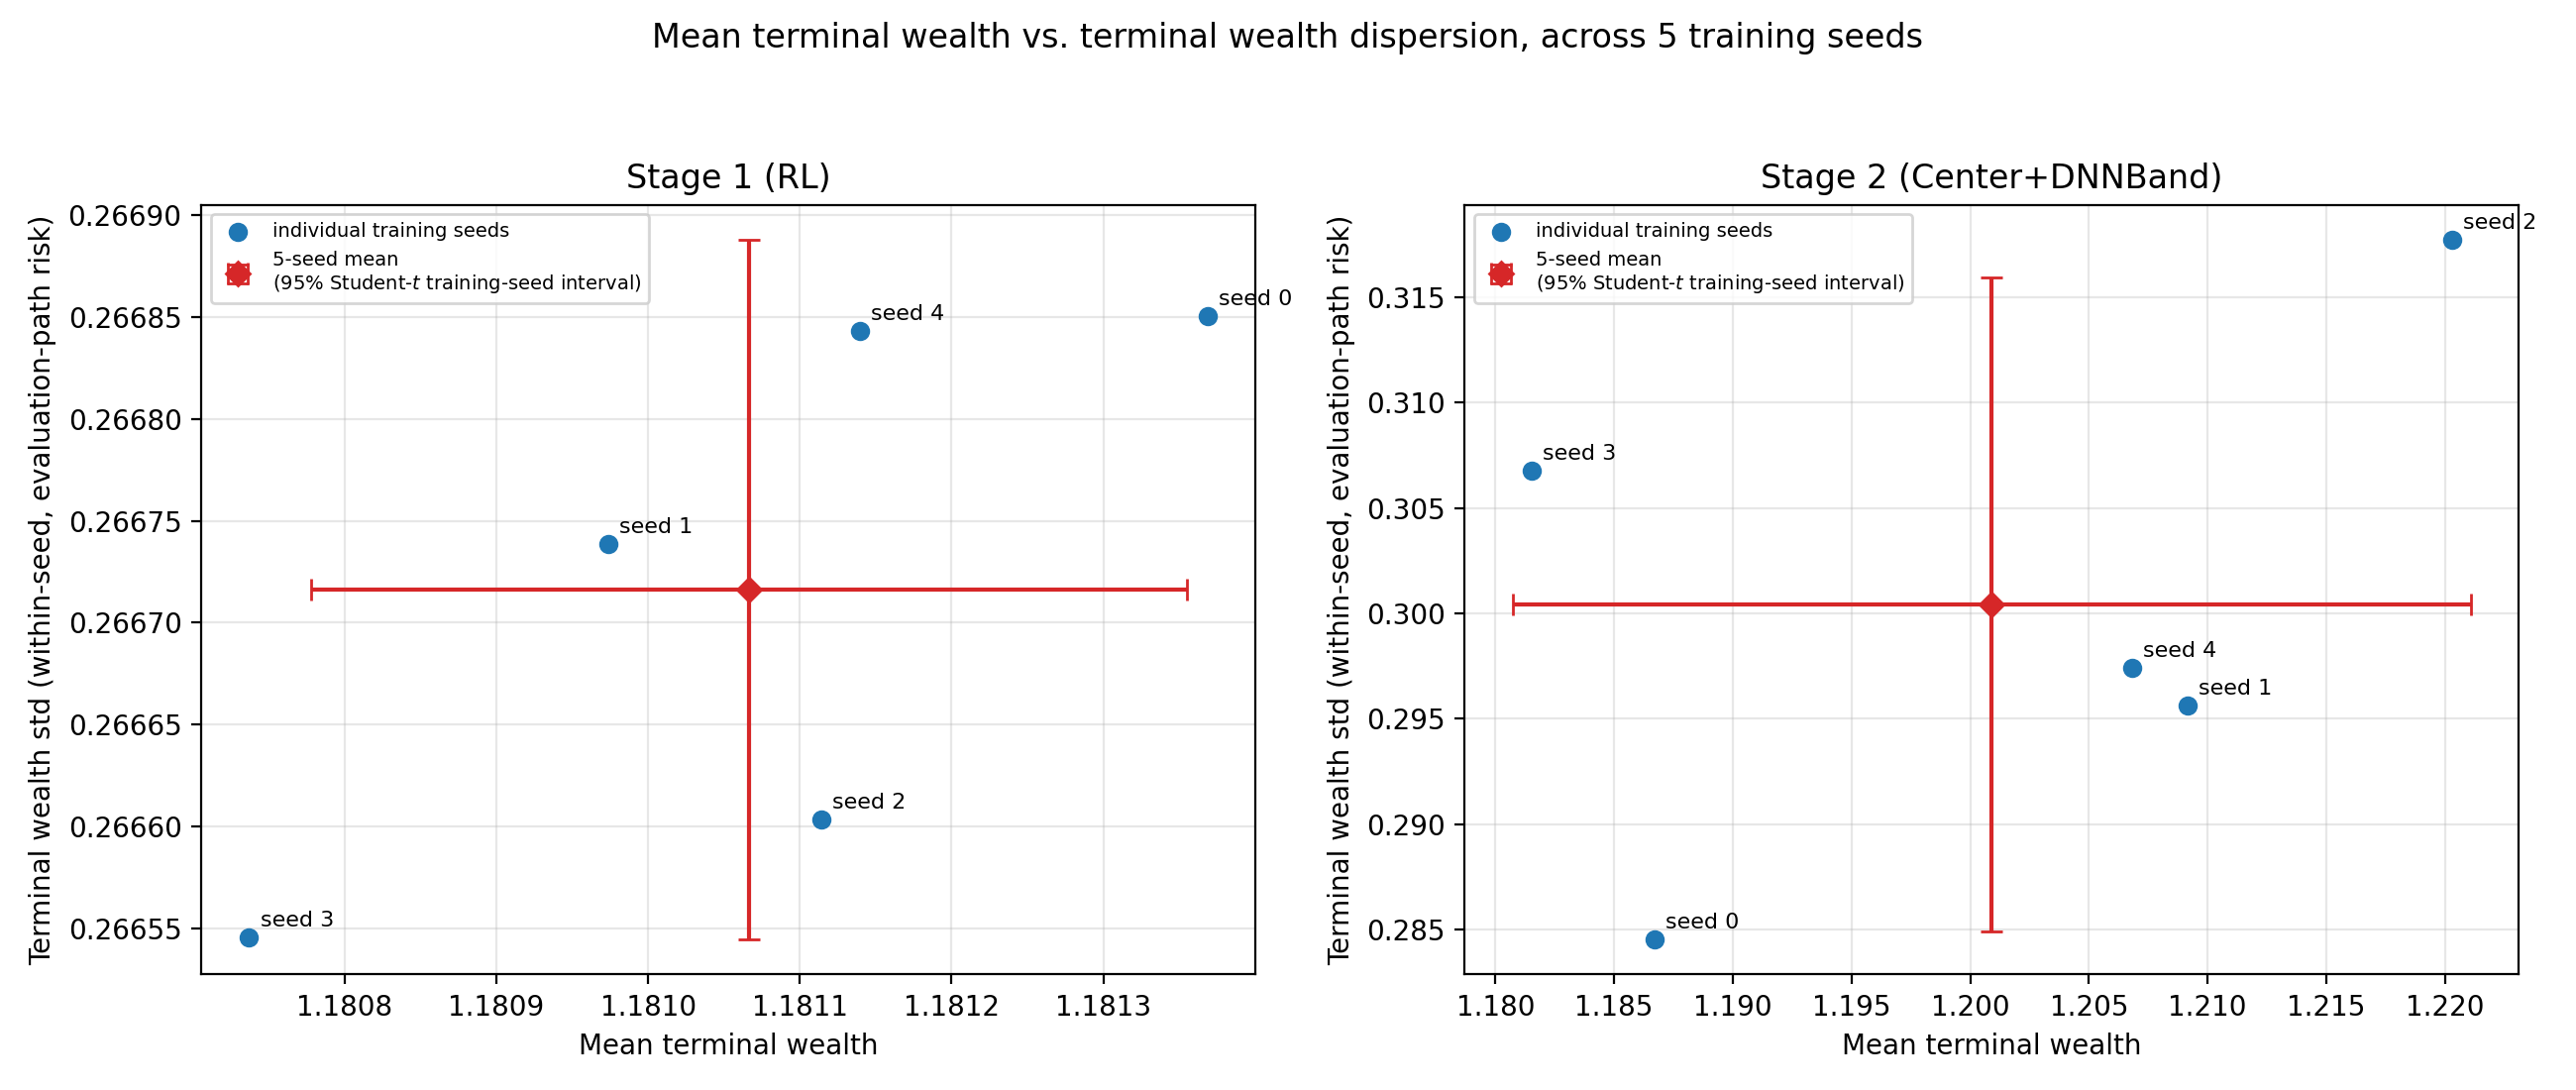
\includegraphics[width=0.92\linewidth]{file/phase1a/fig1_mean_vs_std.png}
\caption{Mean terminal wealth vs.\ within-seed standard deviation, by training seed, with the five-seed mean and its 95\% training-seed interval.}
\end{subfigure}\\[0.6em]
\begin{subfigure}[t]{\textwidth}
\centering
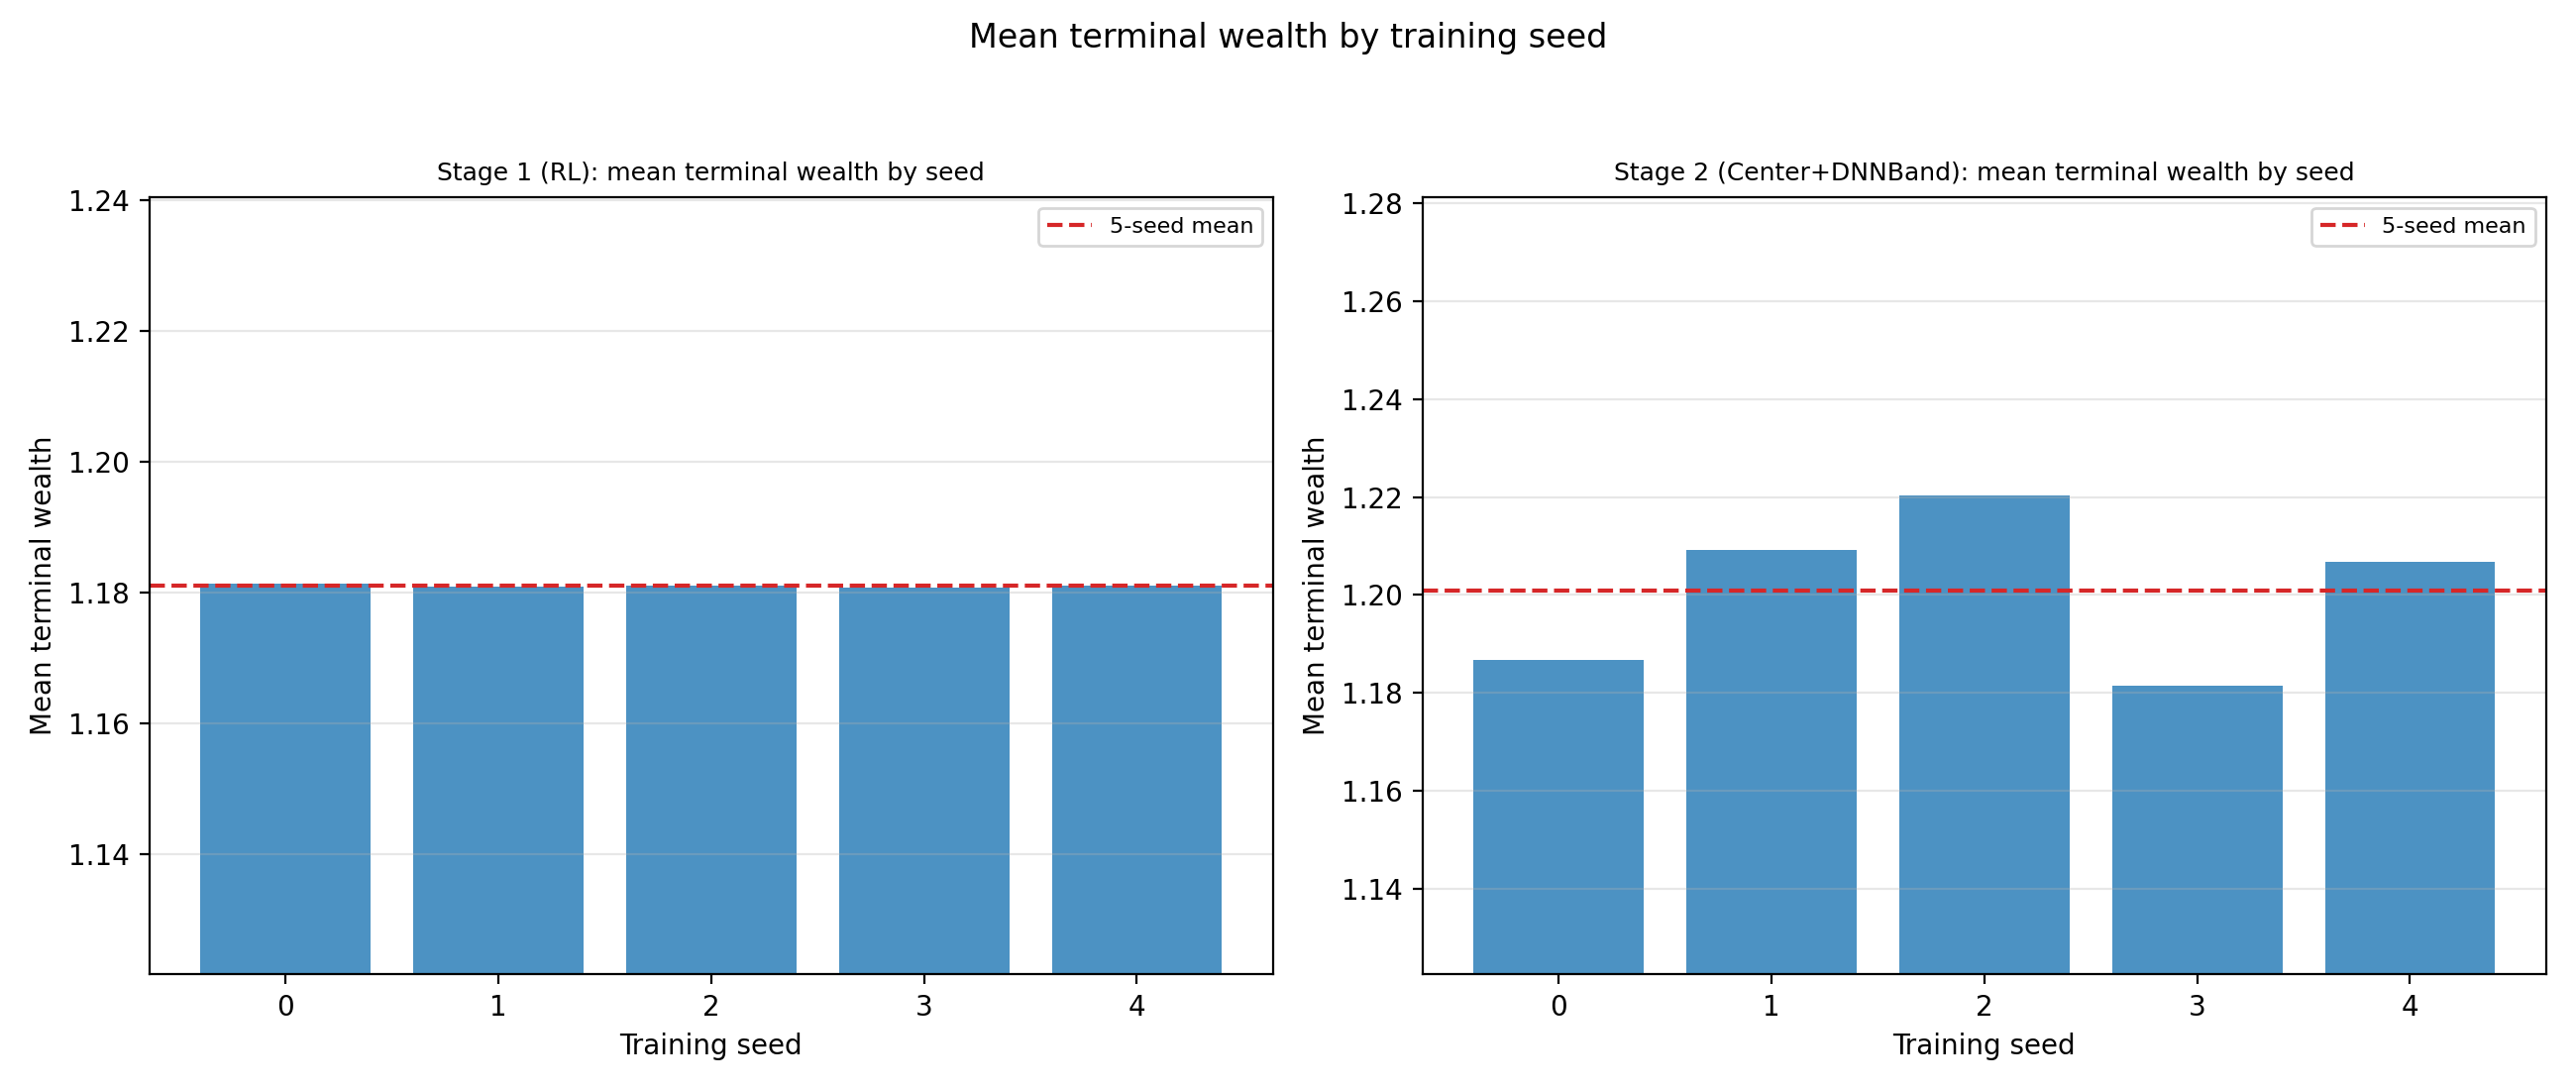
\includegraphics[width=0.92\linewidth]{file/phase1a/fig5_training_seed_variability.png}
\caption{Mean terminal wealth by individual training seed, Stage~1 (left) and Stage~2 (right).}
\end{subfigure}
\caption{Training-seed robustness for the common-covariance HJB-guided policy (Stage~1, left panels of each row) and Center+DNNBand (Stage~2, right panels of each row). Both stages are shown together because the same five training seeds and evaluation design underlie both; Stage~1's near-total overlap of points contrasts with Stage~2's visibly larger spread.}
\label{fig:stage1_common}
\end{figure}

\subsubsection{Exploratory regime-dependent-covariance experiment}
\label{sec:regcov_results}

Table~\ref{tab:regcov_metrics} reports a separate single-seed evaluation
of the regime-dependent-covariance extension. Its purpose is to assess the
implementability of the approximate filtering-and-control architecture; no
multiple-seed inference is drawn from this experiment.

\begin{table}[H]
\centering
\small
\caption{Single-seed exploratory regime-dependent-covariance held-out simulation summary. Not part of the five-seed replication; no training-seed interval is reported.}
\label{tab:regcov_metrics}
\begin{tabular}{lccccc}
\toprule
Method & Mean $X_T$ & Std. $X_T$ & Var. $X_T$ & $\Pbb(X_T\ge z)$ & Mean shortfall \\
\midrule
Equal weight & $1.078$ & $0.271$ & $0.073$ & $0.316$ & $0.180$ \\
Minimum variance & $1.078$ & $0.259$ & $0.067$ & $0.312$ & $0.176$ \\
Approximate HJB RL & $1.132$ & $0.172$ & $0.030$ & $0.342$ & $0.112$ \\
\bottomrule
\end{tabular}
\end{table}

In this single exploratory run, the regime-dependent policy has the highest displayed mean and the lowest dispersion. Its gain in target-hit probability is more modest than in the common-covariance run. This is consistent with the SJM transition-rate mismatch and with the additional approximation in \eqref{eq:effective_wealth_regcov}--\eqref{eq:regcov_f_pde}. The discrete-time Gaussian filtering--correction step is exact for the adopted observation model, but the belief-averaged control layer is a moment-matched approximation with no verification theorem. These numbers demonstrate promising behavior for the implemented surrogate under a single training initialization; they do not prove optimality for the original regime-dependent continuous-time model, and no multi-seed inference or general dominance claim is made for this experiment.

\subsection{Stage 2 results}

Table~\ref{tab:stage2_means} reports the five-seed transaction-cost-aware comparison.

\begin{table}[H]
\centering
\small
\caption{Stage~2 transaction-cost-aware performance across five independent training seeds, $1000$ common evaluation paths per seed. Every entry is a 5-seed mean of the corresponding per-seed statistic (itself already an average over that seed's $1000$ evaluation paths, and additionally over the $252$ within-path steps for Turnover and Band width); bracketed net-terminal-wealth values additionally report the 95\% Student-$t$ interval across the five training seeds. Gross $X_T$ is an accounting decomposition (net wealth plus the transaction cost otherwise deducted, along the same realized trade path), not an independent counterfactual zero-cost re-simulation -- see the metric-definition paragraph above and the discussion following this table. Cum.\ tc is defined as Gross $X_T$ minus Net $X_T$. Band width is a structural quantity defined only for Center+DNNBand; ``--'' denotes not applicable, not zero.}
\label{tab:stage2_means}
\resizebox{\textwidth}{!}{%
\begin{tabular}{lccccccc}
\toprule
Method & Net $X_T$ & Gross $X_T$ & Cum.\ tc & Turnover & Trades & Band width & $\Pbb(X_T\ge z)$ \\
\midrule
Center+DNNBand & $1.2009$ [$1.1807$,\,$1.2211$] & $1.2196$ & $0.0187$ & $0.0397$ & $175.8$ & $1.740$ & $0.490$ \\
CenterOnly, daily & $1.1099$ [$1.1097$,\,$1.1101$] & $1.1595$ & $0.0496$ & $0.1100$ & $252.0$ & -- & $0.426$ \\
CenterOnly, monthly & $1.1229$ [$1.1228$,\,$1.1231$] & $1.1349$ & $0.0120$ & $0.0258$ & $12.0$ & -- & $0.437$ \\
Equal weight, monthly & $1.0372$ (seed-invariant) & $1.0401$ & $0.0029$ & $0.0059$ & $12.0$ & -- & $0.281$ \\
\bottomrule
\end{tabular}}
\end{table}

Gross terminal wealth in Table~\ref{tab:stage2_means} is not an independently re-simulated no-cost scenario: it shares the identical sequence of realized post-trade dollar positions and returns with net terminal wealth, and simply omits the transaction-cost debit at each step, so that by construction gross minus net equals cumulative transaction cost (verified to floating-point precision, Table~\ref{tab:stage2_config}). It does not represent what the policy would have traded, nor what it would have earned, in a world without transaction costs. Table~\ref{tab:full_intervals} in Appendix~\ref{app:paired_full} additionally reports 95\% training-seed intervals for target achievement probability, target MSD, mean shortfall, cumulative transaction cost, turnover, trade count, band width, and mean terminal log-utility with its certainty equivalent (computed from episode-level terminal wealth using the same positivity floor as training, $\epsilon=10^{-10}$) for every Stage~1 and Stage~2 method. Because only Stage~2 was trained against this log-utility objective, the Stage~2 values are objective-consistent evaluation metrics, whereas the Stage~1 values are post-hoc distributional summaries computed under an objective (log utility) different from the one Stage~1 was trained under (precommitted mean--variance).

\begin{table}[H]
\centering
\small
\caption{Selected Stage~2 paired comparisons. Differences are computed at the evaluation-path level within each training seed, averaged within the seed, and then aggregated across five training seeds; 95\% intervals use the Student-$t$ critical value with four degrees of freedom. The Stage~2-versus-Stage~1 row is a descriptive comparison across different terminal objectives, not a claim of dominance (Section~\ref{sec:stage2_vs_stage1}). A complete set of eleven paired comparisons, including all pairwise method differences and gross-minus-net decompositions, is reported in Appendix~\ref{app:paired_full}.}
\label{tab:paired_comparisons}
\begin{tabular}{lccc}
\toprule
Comparison & Mean difference & 95\% training-seed interval & Excludes zero? \\
\midrule
Center+DNNBand $-$ CenterOnly, daily & $0.0910$ & $[0.0709,\,0.1112]$ & yes \\
Center+DNNBand $-$ CenterOnly, monthly & $0.0780$ & $[0.0578,\,0.0981]$ & yes \\
Center+DNNBand $-$ Equal weight, monthly & $0.1637$ & $[0.1436,\,0.1839]$ & yes \\
Stage~2 net $-$ Stage~1 terminal wealth & $0.0198$ & $[-0.0003,\,0.0400]$ & no \\
\bottomrule
\end{tabular}
\end{table}

Center+DNNBand achieved mean net terminal wealth $1.2009$ (95\% training-seed interval $[1.1807,1.2211]$), mean gross terminal wealth $1.2196$, mean cumulative transaction cost $0.0187$, mean turnover $0.0397$, a mean of $175.8$ trades, and mean band width $1.740$. Its paired difference against daily center rebalancing was $0.0910$ with interval $[0.0709,0.1112]$, which excludes zero. The evaluated band-plus-cap Center+DNNBand policy reduced the mean number of trades from $252$ under daily center rebalancing to $175.8$, a reduction of approximately 30\%; because the reported trade count is measured after the evaluation-time leverage cap of \eqref{eq:eval_projection} is applied on top of the learned band, this reduction is attributable to the evaluated band-plus-cap policy rather than to the learned no-trade band alone. This reduction in trade frequency accompanies, but is not shown to causally explain, the net-wealth improvement: separating the contribution of trade frequency from boundary asymmetry, belief conditioning, and time-to-go conditioning would require an ablation study that has not been performed.

\label{sec:stage2_vs_stage1}
The mean descriptive difference between Stage~2 net terminal wealth and Stage~1 terminal wealth was $0.0198$, with a 95\% training-seed interval of $[-0.0003,0.0400]$. Because the interval includes zero and the two stages optimize different terminal objectives (Stage~1 a precommitted mean--variance criterion, Stage~2 a transaction-cost-aware utility objective), this comparison does not establish that Stage~2 dominates Stage~1. It is also notable that, despite its higher mean terminal wealth, Center+DNNBand's target-achievement probability ($0.490$) is lower than Stage~1's ($0.566$): the two stages differ not only in mean level but in the shape of the terminal-wealth distribution relative to the target $z$, so policies should not be ranked by mean terminal wealth alone.

\begin{figure}[H]
\centering
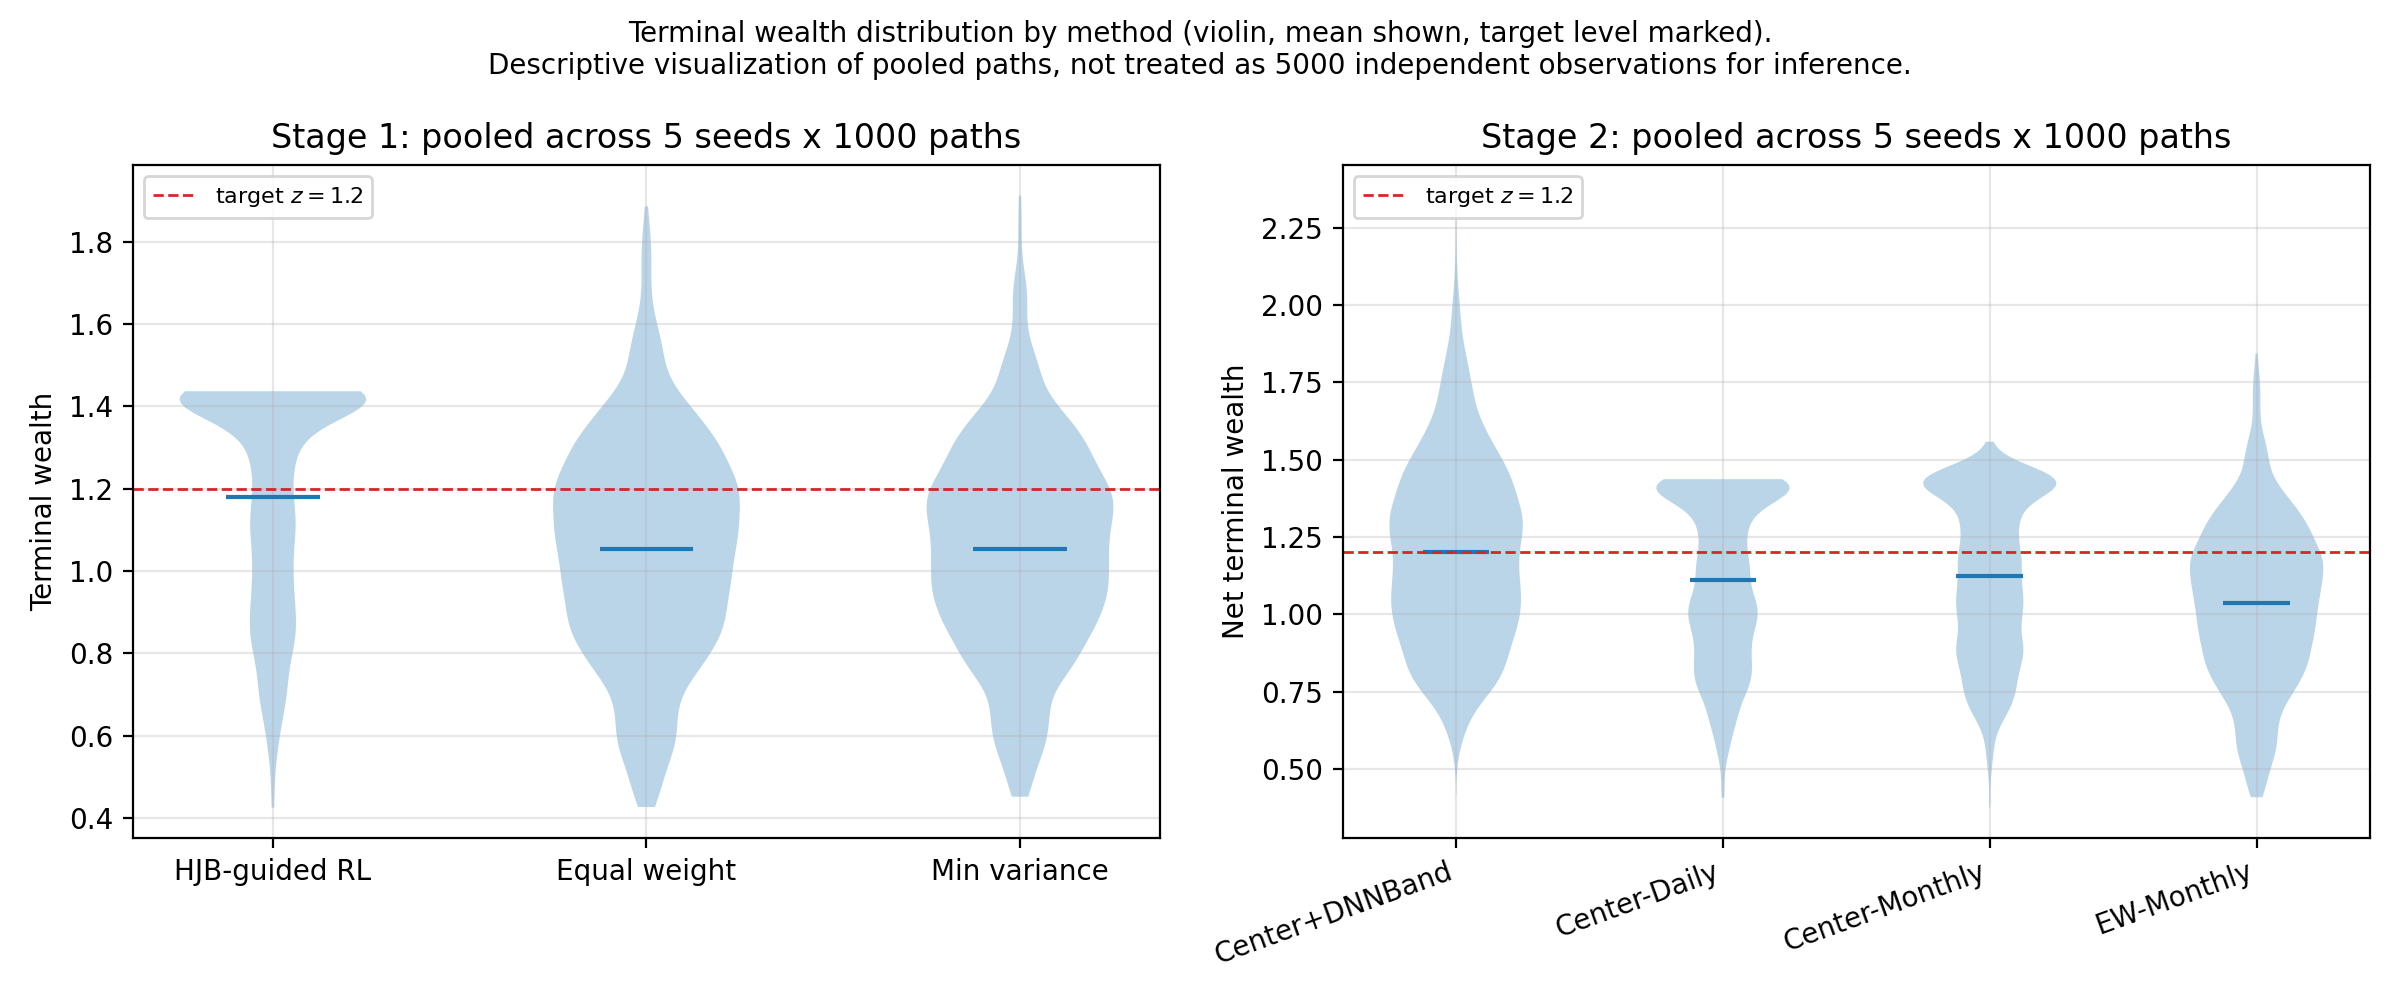
\includegraphics[width=0.85\linewidth]{file/phase1a/fig2_terminal_wealth_distribution.png}
\caption{Terminal wealth distributions pooled across five training seeds and $1000$ evaluation paths each. Left: Stage~1 (RL, equal weight, minimum variance). Right: Stage~2 (Center+DNNBand and the three comparators), net of transaction costs. Horizontal bars mark the pooled mean. These violin plots are descriptive visualizations of the pooled $5\times1000$ observations, not independent samples: the same $1000$ evaluation scenarios recur under all five training seeds, so the pooled distribution mixes within-seed evaluation-path variability with across-seed policy variability rather than depicting $5000$ independent draws.}
\label{fig:stage2_eval}
\end{figure}

\begin{figure}[H]
\centering
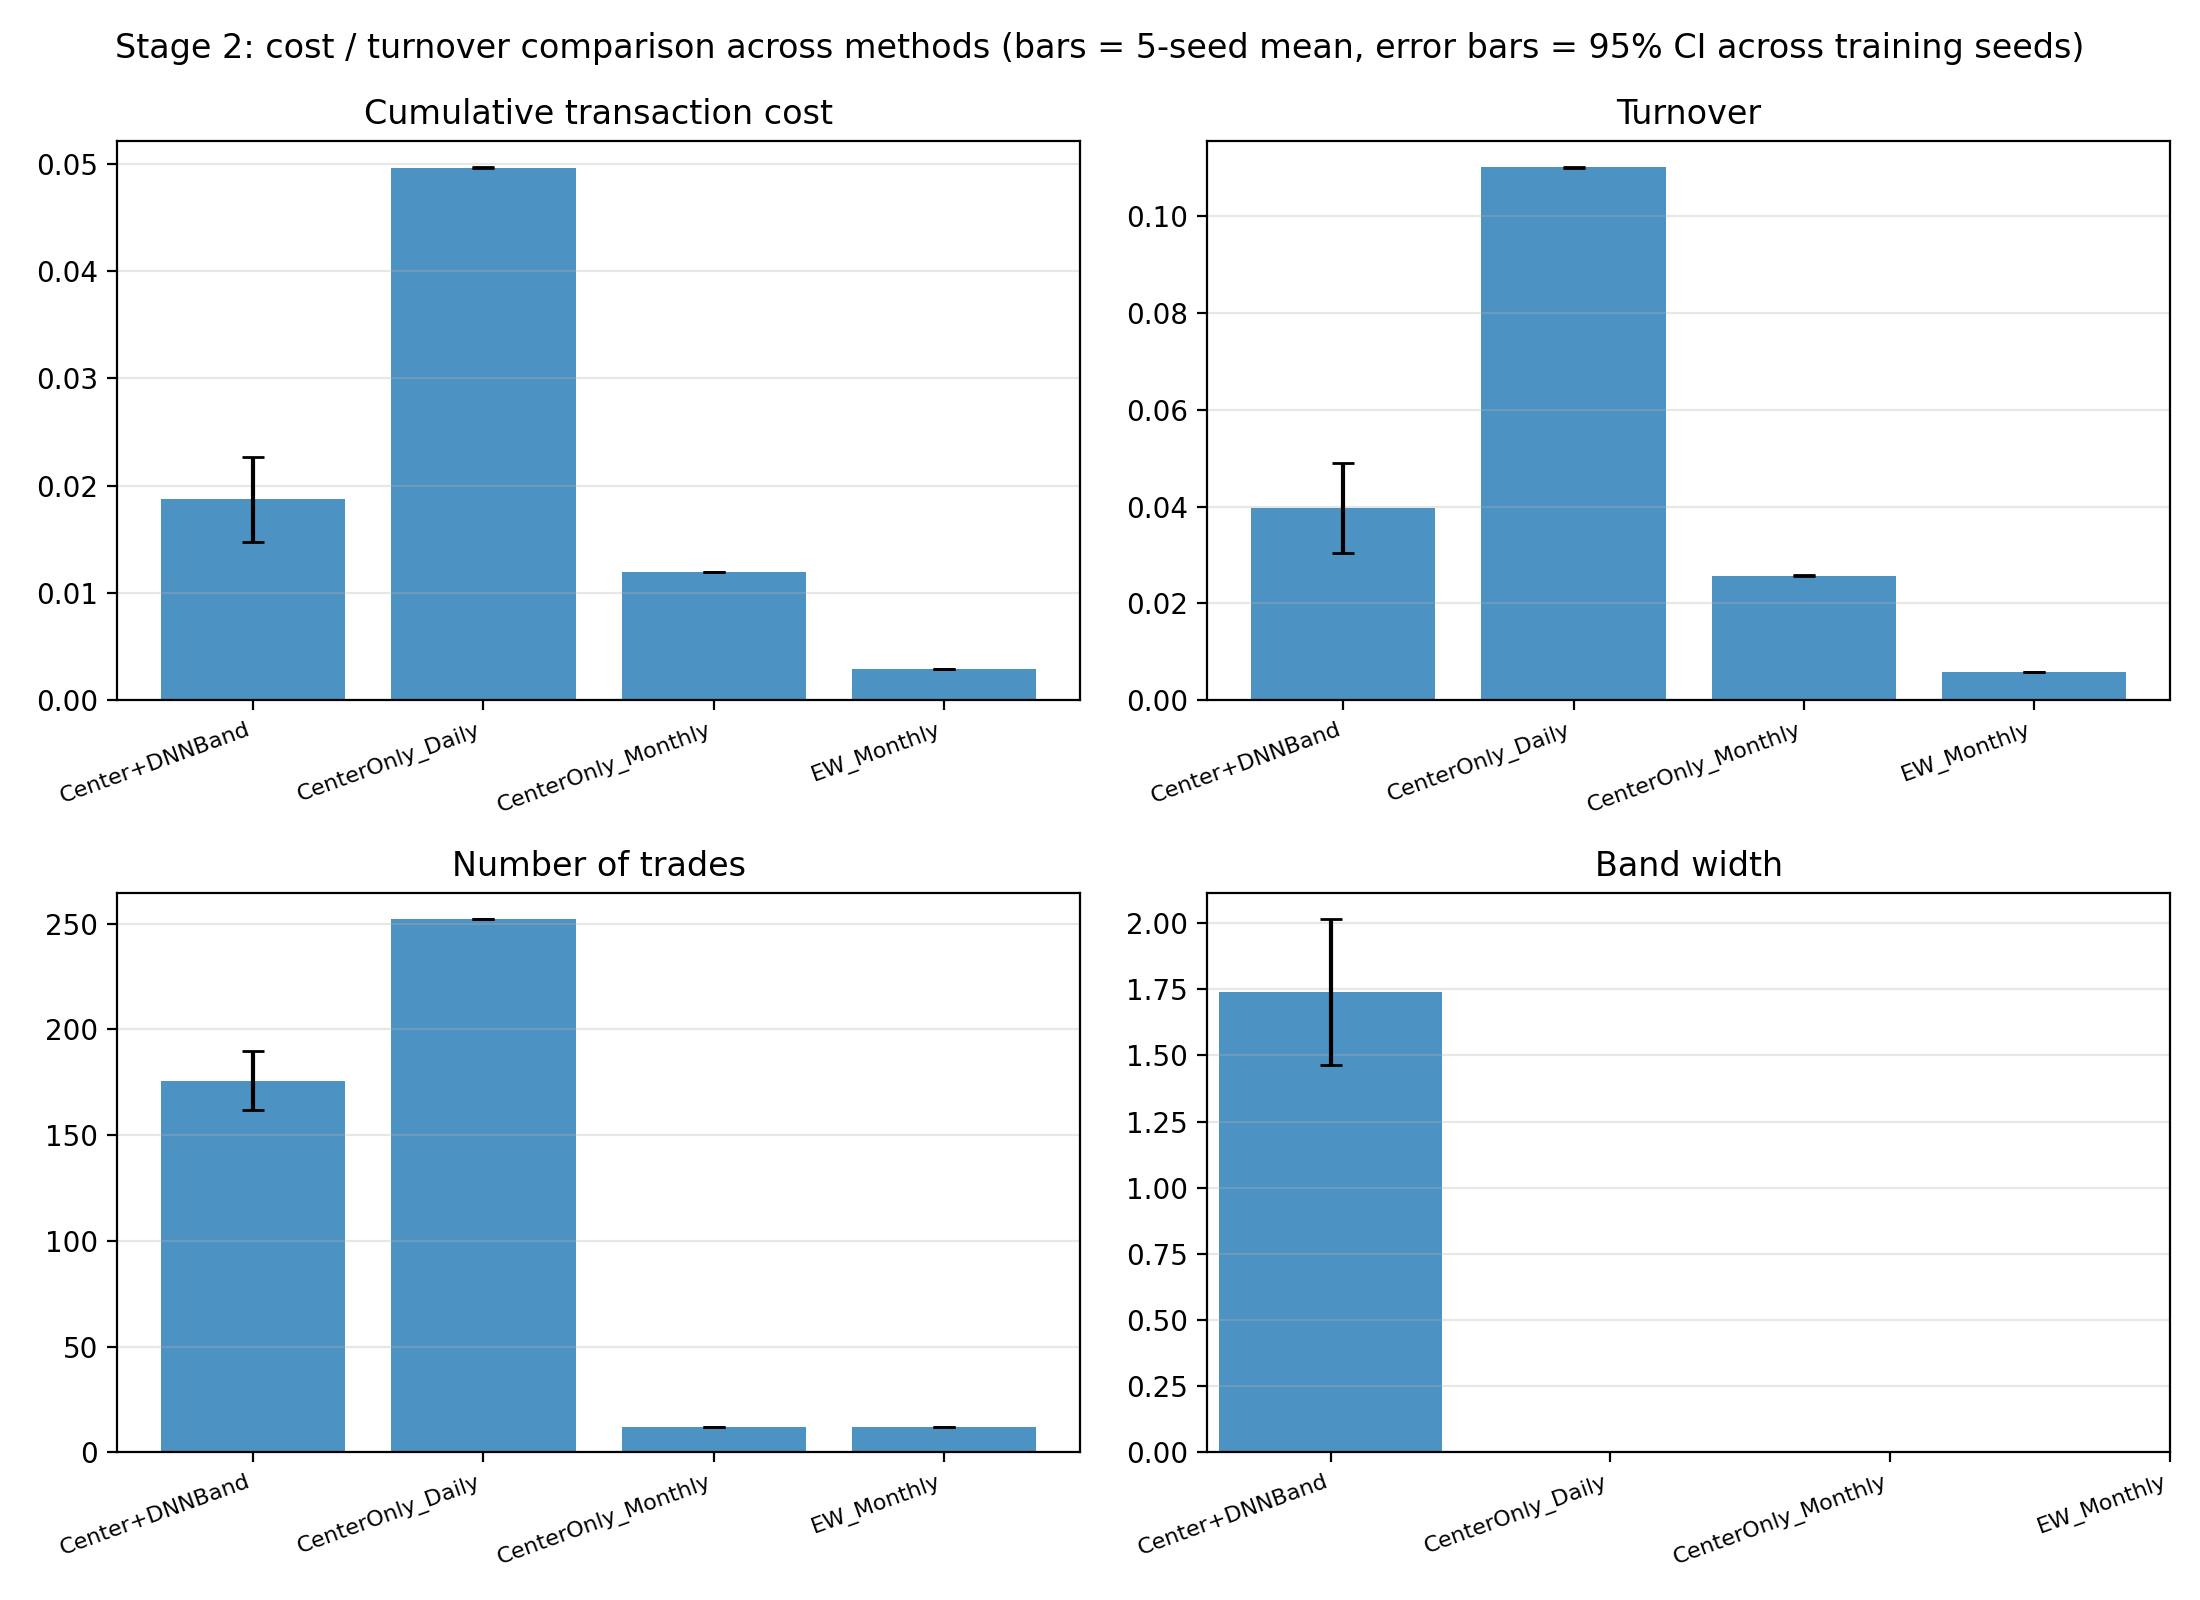
\includegraphics[width=0.95\linewidth]{file/phase1a/fig4_cost_turnover.png}
\caption{Stage~2 cost and turnover comparison across methods: cumulative transaction cost, turnover, trade count, and band width. Bars show the five-seed mean; error bars show the 95\% training-seed interval. Band width bars are blank for methods without a band-width concept (structural, not zero).}
\label{fig:stage2_cost_turnover}
\end{figure}

\section{Discussion}

\subsection{Practical implications}

The results illustrate how an institutional investment rule can separate three economically distinct tasks: estimating the market environment, selecting a frictionless risk exposure, and deciding whether the benefit of rebalancing justifies its cost. The belief state is not merely a forecasting output; it enters the actor, critic, and transaction-cost policy as a decision variable. Likewise, the no-trade region provides an interpretable governance rule: trade only when the current position departs sufficiently from the belief- and horizon-dependent center.

This decomposition also clarifies why reinforcement learning is useful in this setting. The action is naturally a portfolio allocation, the state representation can be constructed to summarize economically relevant information, and the policy must account for the effect of current trading on future wealth and transaction opportunities. Incorporating domain knowledge into the state and policy does more than reduce dimension: the belief has a probabilistic interpretation, the Gaussian Stage~1 actor separates myopic and hedging demand, and the Stage~2 boundary explains when rebalancing is deferred. The same framework permits domain knowledge to enter the objective through target wealth, entropy, turnover, leverage, and transaction-cost terms.

For insurers and pension funds, the target wealth can serve as a reduced-form accumulation or funding objective, while the trading band can reflect an operational preference for stable allocations and controlled turnover. Across the five-seed replication, the evaluated band-plus-cap policy reduced the mean number of trades by approximately 30\% relative to daily center rebalancing (Section~\ref{sec:stage2_vs_stage1}), which can be read as evidence that the framework offers an operational turnover-discipline benefit in addition to its net-performance statement, not only as a net-wealth result. The current results are methodological demonstrations rather than investment recommendations, and actual market impact, transaction-cost nonlinearity, and liability dynamics are not modeled. Their practical value lies in providing a transparent architecture that could later accommodate liability cash flows, capital constraints, prescribed asset limits, and institution-specific transaction budgets.

\subsection{What is exact and what is approximate}

The common-covariance Stage~1 model has the strongest theoretical status: filtering produces an observable diffusion, the entropy-regularized HJB yields the Gaussian optimizer, and the wealth-quadratic ansatz produces exact lower-dimensional coefficient PDEs under the stated regularity conditions. The SJM layer is an estimation methodology that supplies parameters to this filter; it is not part of the control verification theorem.

For regime-dependent covariance, the discrete-time Gaussian prediction--correction filter is exact for the specified hidden Markov observation model, but the belief-averaged effective diffusion and its HJB are moment-matched approximations. For transaction costs, the QVI is the theoretical benchmark and the center-relative critic/intervention actor is exploratory. Center+DNNBand, the reported Direct Boundary policy optimization method, produced a numerically usable pathwise policy across all five training seeds, with a separate terminal objective; it is not a numerical solution of that QVI.

\subsection{Lessons from theory-guided learning}

The experiments suggest an asymmetric role for structural theory. In Stage~1, the common-covariance HJB identifies the Gaussian policy family, the linear dependence of its mean on wealth, the quadratic critic, and the lower-dimensional coefficient functions. These restrictions remove large parts of the learning problem without materially narrowing the theorem-level optimizer. The resulting actor--critic provided usable training and favorable displayed results under both common and regime-dependent covariance. The very small between-seed dispersion in Stage~1 (between-training-seed standard deviation of mean terminal wealth $\approx 0.000232$, against a within-seed evaluation-path standard deviation of $0.267$) is consistent with the stabilizing role of the HJB-restricted actor and critic, although the current experiments do not causally identify that restriction as the source of stability: because a controlled structured-versus-unstructured ablation has not yet been completed, the present evidence does not identify the restrictions themselves as the sole cause of the observed performance.

The Stage~2 experience is different. The QVI identifies the enlarged state, the intervention-versus-continuation logic, and the relevance of a no-trade region, but it does not determine the finite-horizon multidimensional boundary geometry as sharply as the Stage~1 HJB determines the Gaussian actor. Jointly learning the QVI critic, obstacle residual, trigger, and intervention map was unstable. The Direct Boundary architecture instead imposed economically meaningful center-relative no-trade geometry, retained feasibility constraints and pathwise transaction costs, and produced a numerically usable implementation. Consistent with a less sharply identified boundary geometry, the between-training-seed standard deviation of mean net terminal wealth for the end-to-end Stage~1-plus-Stage~2 pipeline (each seed's Stage~2 policy is trained against that same seed's own Stage~1 center checkpoint, so the two stages' initializations are not varied independently) was approximately $0.0163$ -- about $70$ times larger than Stage~1 alone's between-training-seed standard deviation of mean terminal wealth ($\approx 0.000232$) -- indicating materially greater sensitivity to training initialization than Stage~1 under the same five-seed protocol. This reflects the combined pipeline's sensitivity, not an isolated measurement of the Stage~2 optimizer with a fixed Stage~1 center held constant across seeds.

The methodological lesson is not that stronger structural restrictions are always preferable. Theory-guided parametrization is most effective when the underlying control equation identifies the relevant functional form with sufficient precision. When theory supplies only local or qualitative information about a free boundary, a softer inductive bias combined with simulation-based learning may be preferable to enforcing a misspecified low-dimensional geometry. The formula-based QVI actor remains valuable as an interpretable target and potential regularizer, but not yet as the reported optimizer.

\subsection{Sources of performance and model risk}

Performance in the regime-aware pipeline can be affected at five distinct layers:
\begin{enumerate}[label=(\arabic*)]
\item \textbf{Regime identification error:} the SJM may assign observations to economically imperfect states.
\item \textbf{Parameter error:} regime-specific drifts, covariances, and transition intensities may be estimated inaccurately even conditional on the labels.
\item \textbf{Filtering error:} misspecified parameters distort the posterior belief supplied to the controller.
\item \textbf{Control approximation error:} the belief-averaged regime-dependent covariance model may differ from the original partially observed dynamics.
\item \textbf{Optimization error:} actor--critic or boundary training may converge slowly, become unstable, or settle at a poor local solution.
\end{enumerate}
The exploratory regime-dependent experiment combines regime-identification, parameter-estimation, filtering, control-approximation, and optimization errors, so the reported performance difference cannot be attributed to any single layer. The SJM transition-rate mismatch provides direct evidence of parameter risk, while the additional $f_p^2/f$ term and moment matching identify a separate control-model risk. The displayed approximate HJB policy has higher mean terminal wealth and lower dispersion than the static benchmarks, which supports the usefulness of the structural approximation in this setting, but it does not establish universal dominance or isolate the source of the improvement.

The SJM produced a practically usable persistent segmentation in the reported experiment, but the present study does not establish superiority over HMM-based estimation. A controlled comparison should examine label stability, parameter error, posterior filtering accuracy, and downstream portfolio performance under common data and evaluation paths. The current claim is limited to the operational value of combining transparent offline SJM segmentation with online Bayesian belief updating.

Because the reported SJM features are constructed primarily from an equal-weight return index, covariance regimes are identified only indirectly through univariate aggregate-return features. Incorporating cross-sectional dispersion, realized correlation, or rolling covariance features is an important robustness extension, especially because covariance-state variation is a central motivation for the regime-dependent model.

The Stage~2 results have a similarly specific interpretation. Daily rebalancing to the frictionless center has lower mean net wealth than monthly rebalancing, consistent with repeated proportional costs offsetting the marginal tracking benefit. Center+DNNBand has the highest mean net wealth among the reported comparators and reduces mean trade count relative to daily rebalancing, and turnover, cumulative transaction cost, trade count, and band width are now reported as separate summary statistics (Table~\ref{tab:stage2_means}, Figure~\ref{fig:stage2_cost_turnover}) rather than inferred only from net wealth. However, the current evidence does not determine whether the net-wealth difference comes primarily from lower trading frequency, asymmetric boundaries, belief conditioning, or time-to-go conditioning: separating these mechanisms causally requires an ablation analysis that has not been performed.

\subsection{Limitations and robustness status}

The common-covariance Stage~1 and Stage~2 results are verified across five independent training seeds on a common evaluation design (Section~\ref{sec:stage1_results}--\ref{sec:stage2_vs_stage1}). The following limitations remain:
\begin{enumerate}[label=(\arabic*)]
\item Five training seeds are informative about sensitivity to training initialization but remain a small sample; the reported Student-$t$ intervals should not be read as tight population-level confidence statements.
\item The regime-dependent-covariance experiment (Section~\ref{sec:regcov_results}) remains single-seed and exploratory; it is not part of the five-seed replication.
\item Transaction-cost sensitivity (varying $\kappa$ and the leverage cap) has not been examined.
\item An actor-signal ablation separating the martingale and full-horizon terms, and a structured-versus-unstructured policy-class ablation, have not been performed.
\item The evaluation output contains terminal wealth and path-level summary statistics but not complete time-series wealth trajectories, precluding a time-resolved multi-seed wealth-path analysis.
\item A time-resolved leverage-cap saturation measure is not available.
\item Only the combined band width is available; separate lower- and upper-boundary summaries are not reported.
\item Stage~1 and Stage~2 optimize different terminal objectives, so comparisons between them (Section~\ref{sec:stage2_vs_stage1}) are descriptive, not a test of dominance under a common objective.
\item Filtering quality depends on the regime segmentation and parameter estimates, and the estimated transition persistence differs materially from the simulator in the regime-dependent-covariance experiment; the associated control layer is moment-matched rather than exact, and $\widetilde c(p)$ has not been identified from a continuous-time filtering theorem.
\item The attempted QVI-based RL was unstable, and hard componentwise projection in Center+DNNBand is interpretable but does not represent the most general multidimensional intervention geometry.
\item Liabilities, solvency capital, taxes, market impact, and governance constraints are not explicitly modeled.
\end{enumerate}

\subsection{Future research}

The transaction-cost QVI derived in Section~7 provides the theoretical target,
\begin{equation}
\min\{-V_t-\mathcal LV,\ \mathcal MV-V\}=0,
\end{equation}
where $\mathcal M$ accounts for proportional wealth loss and a post-trade target map. The next methodological step is not to formulate this QVI again, but to stabilize its numerical learning: continuation/intervention sampling, obstacle-compatible losses, target networks for $\mathcal M V$, curriculum learning from a Direct Boundary policy, and smooth trigger approximations are natural candidates.

Broader sensitivity to transaction-cost rates, entropy weights, and filtering misspecification, together with ablations separating the effects of the belief state, HJB-guided parametrization, martingale signal, full-horizon residual, symmetric versus asymmetric bands, and QVI-derived priors, remain directions for future work. Stronger benchmarks should include a full-information regime oracle retrained under that information structure, a true-parameter filtered policy, a myopic policy without the belief-hedging term, and a fixed symmetric band. Supplying the true regime directly to a policy trained only on filtered beliefs would instead be an out-of-distribution stress test, not a formal oracle comparison. An actuarial extension should introduce stochastic liability cash flows, funding-ratio or surplus objectives, regulatory capital constraints, and asset eligibility limits so that the portfolio controller becomes a component of a complete ALM problem.

\section{Conclusion}

This paper starts from the view that reinforcement learning is well matched to dynamic portfolio choice when the economically relevant state and admissible policy class are constructed carefully from control theory rather than left unrestricted. The central contribution is a belief-state HJB reduction of partially observed mean--variance control, extended from common to regime-dependent observation covariance; building on this reduction, Stage~1 makes a structure-guided actor--critic operational, and Stage~2 learns a transaction-cost no-trade boundary around the frozen Stage~1 center through Direct Boundary policy optimization. The resulting architecture combines state estimation, sequential control, and rebalancing discipline without treating portfolio selection as an unrestricted state-to-weight prediction problem.

The five-seed common-covariance study gives different robustness conclusions for the two learning stages. Stage~1 converged to nearly identical held-out performance across training seeds, with mean terminal wealth $1.1811$ and very small between-seed dispersion. Center+DNNBand achieved the highest average net terminal wealth among the reported transaction-cost-aware comparators, retained a positive paired difference relative to daily and monthly center rebalancing, and reduced mean trade count by approximately 30\% relative to daily rebalancing under the evaluated band-plus-cap policy; however, it was materially more sensitive to training initialization, and its descriptive net-wealth difference from Stage~1 had a 95\% interval that included zero. The evidence therefore supports robustness relative to the reported Stage~2 comparators, not a claim that Stage~2 statistically dominates the frictionless Stage~1 policy. The regime-dependent-covariance extension remains exploratory and single-seed (Section~\ref{sec:regcov_results}) and is not covered by these five-seed robustness statements. Center+DNNBand is not a numerical solution of the transaction-cost QVI derived in this paper; it is a structurally motivated but separately optimized implementation.

The broader methodological conclusion is that the contribution lies not in deep learning alone, but in selectively using financial structure to determine the information state, restrict policy geometry, and design the objective, while retaining flexible learning where the control theory does not identify the optimal functional form sufficiently sharply. Stage~1 uses strong low-dimensional restrictions because the Gaussian actor and quadratic critic are characterized by the HJB; in Stage~2, the free-boundary geometry is less completely identified, so flexible simulation-based boundary learning provided the usable implementation, while the QVI and center-relative formulas remain theoretical and architectural guides. For actuarial and institutional applications -- where the target wealth can serve as a funding or accumulation objective and the no-trade band as an operational turnover-discipline rule -- this combination of interpretable belief states, structured policies, and transaction-aware rebalancing offers a tractable portfolio-control building block, not a complete asset--liability management solution; a full ALM extension would additionally require stochastic liabilities, capital constraints, and institution-specific admissibility rules (Section~\ref{sec:actuarial}).

\section*{Acknowledgment}

Generative AI tools were used to assist with language editing, document organization, and review. Responsibility for verifying the mathematical derivations, numerical results, originality, and references remains with the author.

\appendix

\section{Explicit QVI Continuation Coefficients}
\label{app:qvi_coefficients}

For compactness, suppress the arguments $(p,\bw)$ and define
\begin{equation}
s=\|\bar\sigma\|^2,\quad
q=\|\beta\|^2,\quad
R=DD^\top,\quad
c_p=\bar\sigma^\top\beta,\quad
c_w=D\bar\sigma,\quad
c_{pw}=D\beta.
\end{equation}
The generator associated with \eqref{eq:no_trade_dynamics} is
\begin{align}
\mathcal LV={}&x\bar\mu V_x+\mu_pV_p+b_w^\top\nabla_wV
+\tfrac12x^2sV_{xx}+\tfrac12qV_{pp}
+\tfrac12\operatorname{tr}(R\nabla^2_{ww}V) \notag\\
&+xc_pV_{xp}+xc_w^\top\nabla_wV_x
+c_{pw}^\top\nabla_wV_p.
\end{align}
Substitution of \eqref{eq:tc_ansatz} into \eqref{eq:phi_decomposition} gives
\begin{align}
\Phi_2={}&-A_t-2\bar\mu A-sA-\mu_pA_p-b_w^\top\nabla_wA
-\tfrac12qA_{pp}-\tfrac12\operatorname{tr}(R\nabla^2_{ww}A) \notag\\
&-2c_pA_p-2c_w^\top\nabla_wA-c_{pw}^\top\nabla_wA_p,
\label{eq:phi2}\\
\Phi_1={}&-B_t-\bar\mu(B+2\omega A)-2\omega sA
-\mu_pB_p-b_w^\top\nabla_wB
-\tfrac12qB_{pp}-\tfrac12\operatorname{tr}(R\nabla^2_{ww}B) \notag\\
&-c_p(B_p+2\omega A_p)
-c_w^\top(\nabla_wB+2\omega\nabla_wA)
-c_{pw}^\top\nabla_wB_p,
\label{eq:phi1}\\
\Phi_0={}&-C_t-\omega\bar\mu B-\omega^2sA
-\mu_pC_p-b_w^\top\nabla_wC
-\tfrac12qC_{pp}-\tfrac12\operatorname{tr}(R\nabla^2_{ww}C) \notag\\
&-\omega c_pB_p-\omega c_w^\top\nabla_wB
-c_{pw}^\top\nabla_wC_p.
\label{eq:phi0}
\end{align}
Equations \eqref{eq:phi2}--\eqref{eq:phi0} show why a third coefficient $B$ is required: even if $B(T,p,\bw)=0$, the terms proportional to $\omega A$ act as sources for the linear equation away from maturity.

\section{Center-Relative QVI Critic and Intervention Actor}
\label{app:qvi_basis}

Let $\tau=T-t$, $\delta=\bw-\bw^{\mathrm{ref}}(t,p)$, and
\begin{equation}
\|\delta\|_{M(p)}^2=\delta^\top M(p)\delta,
\end{equation}
where $M(p)$ may be $I$, $\overline\bSigma(p)^{-1}$, or a diagonal inverse-variance metric. A low-dimensional critic consistent with positivity of $A$ and the parity of the coefficient equations is
\begin{align}
A_\theta(\tau,p,\delta)
&=\exp\left(a_0(\tau,p)+a_2(\tau,p)\|\delta\|_{M(p)}^2
+a_4(\tau,p)\|\delta\|_{M(p)}^4\right),\\
B_\theta(\tau,p,\delta)
&=b_1(\tau,p)^\top\delta
+b_3(\tau,p)^\top\delta\,\|\delta\|_{M(p)}^2,\\
C_\theta(\tau,p,\delta)
&=c_0(\tau,p)+c_2(\tau,p)\|\delta\|_{M(p)}^2
+c_4(\tau,p)\|\delta\|_{M(p)}^4.
\end{align}
Each coefficient surface in $(\tau,p)$ can be represented by a low-order polynomial, as in Stage~1. The intervention actor may be written
\begin{equation}
\Gamma_\phi(t,p,\bw)
=\bw+G_\phi(\tau,p,\delta)
=\bw^{\mathrm{ref}}(t,p)+\delta+G_\phi(\tau,p,\delta),
\end{equation}
with a radial--directional model
\begin{equation}
G_\phi=-s_\phi(\tau,p,\delta)\delta+R_\phi(\tau,p,\delta),
\qquad
s_\phi=\operatorname{sigmoid}\left(
\eta_0(\tau,p)+\eta_2(\tau,p)\|\delta\|_{M(p)}^2
+\eta_4(\tau,p)\|\delta\|_{M(p)}^4
\right).
\end{equation}
The radial first model sets $R_\phi\equiv0$, so $s_\phi=0$ gives no trade and $s_\phi=1$ moves directly to the normalized reference center. This ensures $G_\phi(\tau,p,0)=0$ and biases interventions toward that center. A feasibility layer can enforce simplex, box, or leverage constraints. Because the implemented center \eqref{eq:wealth_dependent_center} depends on wealth, this appendix basis is an architectural approximation and does not claim exact closure after the wealth-dependent change of coordinates.

For the cost-minimization convention, define
\begin{equation}
R_{\mathrm{cont}}=-V_{\theta,t}-\mathcal LV_\theta,
\qquad
R_{\mathrm{obs}}=\mathcal M_\phi V_\theta-V_\theta.
\end{equation}
The exact QVI requires
\begin{equation}
R_{\mathrm{cont}}\ge0,\qquad R_{\mathrm{obs}}\ge0,\qquad
R_{\mathrm{cont}}R_{\mathrm{obs}}=0.
\end{equation}
A soft residual objective may combine terminal supervision with penalties for negative continuation/obstacle residuals and complementarity:
\begin{equation}
\mathcal L_{\mathrm{QVI}}
=\mathcal L_{\mathrm{terminal}}
+\lambda_c\E[(R_{\mathrm{cont}}^-)^2]
+\lambda_o\E[(R_{\mathrm{obs}}^-)^2]
+\lambda_{co}\E[(R_{\mathrm{cont}}R_{\mathrm{obs}})^2],
\end{equation}
where $r^-=\min(r,0)$. This residual objective defines the QVI-based alternative considered in
the study. Under the tested optimization scheme, simultaneous fitting of
the residuals and intervention policy was unstable; the reported Stage~2
results therefore use Direct Boundary policy optimization.

\section{Complete Paired Comparisons and Metric Intervals}
\label{app:paired_full}

Table~\ref{tab:paired_full} reports all eleven Stage~2 paired comparisons computed for the five-seed replication, extending the four comparisons selected for the main text (Table~\ref{tab:paired_comparisons}). Methodology is identical: differences are computed at the evaluation-path level within each of the five training seeds, averaged within the seed, and then aggregated across seeds using the Student-$t$ critical value with four degrees of freedom. Rows marked ``descriptive'' compare methods with different rebalancing rules or, in the Stage~2-versus-Stage~1 case, different terminal objectives; they are not dominance claims.

\begin{table}[H]
\centering
\small
\caption{Complete set of paired comparisons, $5$ training seeds $\times$ $1000$ evaluation paths per seed.}
\label{tab:paired_full}
\begin{tabular}{lcccc}
\toprule
Comparison & Mean diff.\ & 95\% interval & Excl.\ zero? & Type \\
\midrule
Stage~2 net $-$ Stage~1 terminal wealth & $0.0198$ & $[-0.0003,\,0.0400]$ & no & descriptive \\
Gross $-$ net, Center+DNNBand & $0.0187$ & $[0.0148,\,0.0227]$ & yes & cost decomposition \\
Gross $-$ net, CenterOnly daily & $0.0496$ & $[0.0496,\,0.0497]$ & yes & cost decomposition \\
Gross $-$ net, CenterOnly monthly & $0.0120$ & $[0.0120,\,0.0120]$ & yes & cost decomposition \\
Gross $-$ net, EW monthly & $0.0029$ & $[0.0029,\,0.0029]$ & yes & cost decomposition \\
Center+DNNBand $-$ CenterOnly daily & $0.0910$ & $[0.0709,\,0.1112]$ & yes & descriptive \\
Center+DNNBand $-$ CenterOnly monthly & $0.0780$ & $[0.0578,\,0.0981]$ & yes & descriptive \\
Center+DNNBand $-$ EW monthly & $0.1637$ & $[0.1436,\,0.1839]$ & yes & descriptive \\
CenterOnly daily $-$ CenterOnly monthly & $-0.0131$ & $[-0.0131,\,-0.0130]$ & yes & descriptive \\
CenterOnly daily $-$ EW monthly & $0.0727$ & $[0.0725,\,0.0729]$ & yes & descriptive \\
CenterOnly monthly $-$ EW monthly & $0.0858$ & $[0.0856,\,0.0860]$ & yes & descriptive \\
\bottomrule
\end{tabular}
\end{table}

Table~\ref{tab:full_intervals} reports 95\% Student-$t$ training-seed intervals for evaluation metrics not already fully tabulated with intervals in the main text (Tables~\ref{tab:common_metrics} and \ref{tab:stage2_means} report only the terminal-wealth interval). Mean terminal log-utility and its certainty equivalent are reported for the HJB-guided Stage~1 policy and all four Stage~2 comparators, but not for the static Stage~1 equal-weight and minimum-variance baselines. Only the Stage~2 values are objective-consistent, since Stage~2 is trained directly against this log-utility objective; the Stage~1 value is a post-hoc distributional summary evaluated under an objective different from the precommitted mean--variance criterion Stage~1 was actually trained under, and should not be read as evidence about Stage~1's performance under its own objective. ``--'' denotes a metric not applicable to that method (e.g.\ band width for non-DNN-band Stage~2 comparators, or Stage~2-specific cost/turnover metrics for the Stage~1 policies, which do not trade with proportional cost in the Stage~1 evaluation).

\begin{table}[H]
\centering
\footnotesize
\caption{Distributional metrics and post-hoc log-utility summaries, 5-seed mean with 95\% Student-$t$ interval across training seeds (Stage~1: within-seed statistic over $1000$ paths; Stage~2: as Table~\ref{tab:stage2_means}). Target MSD and mean shortfall are derived from evaluation terminal wealth, not native solver outputs. Mean terminal utility and its log-utility certainty equivalent are computed from episode-level terminal wealth using $U(x)=\log(\max(x,10^{-10}))$, the exact positivity floor used in training; these are objective-consistent only for Stage~2, which was trained against this objective, and are post-hoc distributional summaries (not objective-consistent) for the Stage~1 row, which was trained under a precommitted mean--variance criterion.}
\label{tab:full_intervals}
\resizebox{\textwidth}{!}{%
\begin{tabular}{llcccc}
\toprule
Stage & Method & $\Pbb(X_T\ge z)$ & Target MSD & Mean shortfall & Mean terminal utility (cert.\ equiv.) \\
\midrule
1 & HJB-guided RL & $0.5664$ [$0.5657$,\,$0.5671$] & $0.0714$ [$0.0713$,\,$0.0715$] & $0.1247$ [$0.1246$,\,$0.1248$] & $0.1358$ [$0.1356$,\,$0.1361$] ($1.1455$) \\
1 & Equal weight & $0.3040$ (seed-invariant) & $0.0934$ (seed-invariant) & $0.1943$ (seed-invariant) & -- \\
1 & Minimum variance & $0.2910$ (seed-invariant) & $0.0874$ (seed-invariant) & $0.1913$ (seed-invariant) & -- \\
2 & Center+DNNBand & $0.4902$ [$0.4699$,\,$0.5105$] & $0.0905$ [$0.0810$,\,$0.1000$] & $0.1229$ [$0.1126$,\,$0.1332$] & $0.1509$ [$0.1338$,\,$0.1679$] ($1.1629$) \\
2 & CenterOnly, daily & $0.4260$ [$0.4242$,\,$0.4278$] & $0.0780$ [$0.0780$,\,$0.0781$] & $0.1633$ [$0.1632$,\,$0.1633$] & $0.0722$ [$0.0720$,\,$0.0724$] ($1.0749$) \\
2 & CenterOnly, monthly & $0.4368$ [$0.4362$,\,$0.4374$] & $0.0739$ [$0.0738$,\,$0.0739$] & $0.1538$ [$0.1538$,\,$0.1539$] & $0.0859$ [$0.0858$,\,$0.0861$] ($1.0897$) \\
2 & Equal weight, monthly & $0.2810$ (seed-invariant) & $0.0970$ (seed-invariant) & $0.2049$ (seed-invariant) & $0.0001$ (seed-invariant) ($1.0001$) \\
\bottomrule
\end{tabular}}
\end{table}

\begin{table}[H]
\centering
\footnotesize
\caption{Stage~2 cost/turnover metrics, 5-seed mean with 95\% Student-$t$ interval across training seeds; each per-seed value is already averaged over $1000$ evaluation paths and, for turnover and band width, over the $252$ within-path steps (see the metric-definition paragraph, Section~\ref{sec:experimental_design}).}
\label{tab:full_intervals_cost}
\begin{tabular}{lcccc}
\toprule
Method & Cumulative tc & Turnover & Trade count & Band width \\
\midrule
Center+DNNBand & $0.0187$ [$0.0148$,\,$0.0227$] & $0.0397$ [$0.0303$,\,$0.0491$] & $175.8$ [$162.0$,\,$189.5$] & $1.740$ [$1.465$,\,$2.015$] \\
CenterOnly, daily & $0.0496$ [$0.0496$,\,$0.0497$] & $0.1100$ [$0.1099$,\,$0.1100$] & $252.0$ (seed-invariant) & -- \\
CenterOnly, monthly & $0.0120$ (seed-invariant) & $0.0258$ (seed-invariant) & $12.0$ (seed-invariant) & -- \\
Equal weight, monthly & $0.0029$ (seed-invariant) & $0.0059$ (seed-invariant) & $12.0$ (seed-invariant) & -- \\
\bottomrule
\end{tabular}
\end{table}

\section{Code and Reproducibility Materials}

The implementation of the Stage~1 and Stage~2 methods, the experiment
configurations, and the scripts used to generate the reported tables and
figures are available from the author upon reasonable request. All numerical
experiments use synthetic data generated from the models specified in the
paper.

The five-seed common-covariance experiments are reproducible from the
corresponding configurations and evaluation outputs. For the exploratory
regime-dependent-covariance experiment, the exact rolling-feature windows,
feature-normalization statistics, and estimation-sample seed are not
documented. That experiment is therefore presented as exploratory rather
than as a fully reproducible numerical benchmark.

\begin{thebibliography}{99}

\bibitem{aydinhan2024}
A.~O. Ayd{\i}nhan, P.~N. Kolm, J.~M. Mulvey, and Y.~Shu.
Identifying patterns in financial markets: extending the statistical jump model for regime identification.
\emph{Annals of Operations Research}, 2024.
doi:10.1007/s10479-024-06035-z.

\bibitem{davisnorman1990}
M.~H.~A. Davis and A.~R. Norman.
Portfolio selection with transaction costs.
\emph{Mathematics of Operations Research}, 15(4):676--713, 1990.

\bibitem{elliott2010}
R.~J. Elliott, T.~K. Siu, and L.~Badescu.
On mean--variance portfolio selection under a hidden Markovian regime-switching model.
\emph{Economic Modelling}, 27(3):678--686, 2010.

\bibitem{jiazhope2022}
Y.~Jia and X.~Y. Zhou.
Policy evaluation and temporal-difference learning in continuous time and space: A martingale approach.
\emph{Journal of Machine Learning Research}, 23:1--55, 2022.

\bibitem{jiazhopepg2022}
Y.~Jia and X.~Y. Zhou.
Policy gradient and actor--critic learning in continuous time and space: Theory and algorithms.
\emph{Journal of Machine Learning Research}, 23:1--50, 2022.

\bibitem{han2018}
J.~Han, A.~Jentzen, and W.~E.
Solving high-dimensional partial differential equations using deep learning.
\emph{Proceedings of the National Academy of Sciences}, 115(34):8505--8510, 2018.

\bibitem{krishnamurthy2016}
V.~Krishnamurthy.
\emph{Partially Observed Markov Decision Processes: From Filtering to Controlled Sensing}.
Cambridge University Press, 2016.

\bibitem{magill1976}
M.~J.~P. Magill and G.~M. Constantinides.
Portfolio selection with transactions costs.
\emph{Journal of Economic Theory}, 13(2):245--263, 1976.

\bibitem{mulvey2020}
J.~M. Mulvey, Y.~Sun, M.~Wang, and J.~Ye.
Optimizing a portfolio of mean-reverting assets with transaction costs via a feedforward neural network.
\emph{Quantitative Finance}, 2020. doi:10.1080/14697688.2020.1729994.

\bibitem{rieder2005}
U.~Rieder and N.~B{\"a}uerle.
Portfolio optimization with unobservable Markov-modulated drift process.
\emph{Journal of Applied Probability}, 42(2):362--378, 2005.

\bibitem{shrevesoner1994}
S.~E. Shreve and H.~M. Soner.
Optimal investment and consumption with transaction costs.
\emph{The Annals of Applied Probability}, 4(3):609--692, 1994.

\bibitem{sirignano2018}
J.~Sirignano and K.~Spiliopoulos.
DGM: A deep learning algorithm for solving partial differential equations.
\emph{Journal of Computational Physics}, 375:1339--1364, 2018.

\bibitem{taksar1988}
M.~Taksar, M.~J. Klass, and D.~Assaf.
A diffusion model for optimal portfolio selection in the presence of brokerage fees.
\emph{Mathematics of Operations Research}, 13(2):277--294, 1988.

\bibitem{wangzhou2020}
H.~Wang and X.~Y. Zhou.
Continuous-time mean--variance portfolio selection: A reinforcement learning framework.
\emph{Mathematical Finance}, 30(4):1273--1308, 2020.

\bibitem{wangzariphopoulouzhou2020}
H.~Wang, T.~Zariphopoulou, and X.~Y. Zhou.
Reinforcement learning in continuous time and space: A stochastic control approach.
\emph{Journal of Machine Learning Research}, 21(198):1--34, 2020.

\bibitem{wu2024}
B.~Wu and L.~Li.
Reinforcement learning for continuous-time mean--variance portfolio selection in a regime-switching market.
\emph{Journal of Economic Dynamics and Control}, 158:104787, 2024.

\bibitem{wonham1964}
W.~M. Wonham.
Some applications of stochastic differential equations to optimal nonlinear filtering.
\emph{Journal of the Society for Industrial and Applied Mathematics, Series A: Control}, 2(3):347--369, 1964.

\bibitem{xiongzhou2007}
J.~Xiong and X.~Y. Zhou.
Mean--variance portfolio selection under partial information.
\emph{SIAM Journal on Control and Optimization}, 46(1):156--175, 2007.

\bibitem{zhouyin2003}
X.~Y. Zhou and G.~Yin.
Markowitz's mean--variance portfolio selection with regime switching: A continuous-time model.
\emph{SIAM Journal on Control and Optimization}, 42(4):1466--1482, 2003.

\end{thebibliography}

\end{document}